% ----------------------- TODO ---------------------------
% Diese Daten müssen pro Blatt angepasst werden:
\newcommand{\NUMBER}{1}
\newcommand{\EXERCISES}{5}
% Diese Daten müssen einmalig pro Vorlesung angepasst werden:
\newcommand{\COURSE}{HPC Lab - Assignment 3}

\newcommand{\STUDENTA}{Zirong Cai}
\newcommand{\STUDENTB}{Phuong Nguyen}
\title{\vspace{-2em} Assignment 3 - MPI \vspace{-0.5em}}
\author{ \STUDENTA, \STUDENTB}
\date{\today {\vspace{-1cm}}}

% ----------------------- TODO ---------------------------

\documentclass[article]{scrartcl}

\usepackage[utf8]{inputenc}
\usepackage[ngerman]{babel}
\usepackage{amsmath}
\usepackage{amssymb}
\usepackage{fancyhdr}
\usepackage{color}
\usepackage{graphicx}
\usepackage{lastpage}
\usepackage{listings}
\usepackage{tikz}
\usepackage{pdflscape}
\usepackage{subfigure}
\usepackage{float}
\usepackage{polynom}
\usepackage{hyperref}
\usepackage{tabularx}
\usepackage{forloop}
\usepackage{geometry}
\usepackage{listings}
\usepackage{caption}
\usepackage{fancybox}
\usepackage{tikz}
\usepackage{algpseudocode,algorithm,algorithmicx}
%\usepackage{biblatex}
\usepackage{cite}

\setkomafont{title}{\normalsize}
\setkomafont{author}{\small}
\setkomafont{date}{\small}
\setkomafont{section}{\normalfont \normalsize \textbf}
\setkomafont{subsection}{\normalfont}
\renewcommand*{\thesubsection}{\alph{subsection}}

\setkomafont{subsubsection}{\normalfont\itshape}

\lstset { %
    language=C++,
    backgroundcolor=\color{black!5}, % set backgroundcolor
    basicstyle=\footnotesize,% basic font setting
}
%\captionsetup[lstlisting]{ format=listings, labelfont=white, textfont=white}

%Definiere Let-Command für algorithmen
%\newcommand*\Let[2]{\State #1 $\gets$ #2}

%\input kvmacros

%Größe der Ränder setzen
\geometry{a4paper,left=3cm, right=3cm, top=3cm, bottom=3cm}

%Kopf- und Fußzeile
\pagestyle {fancy}
\fancyhead[L]{\STUDENTA, \STUDENTB}
\fancyhead[R]{\COURSE}

\fancyfoot[L]{}
\fancyfoot[R]{Page \thepage /\pageref*{LastPage}}

\begin{document}


\maketitle
\thispagestyle{fancy}

%% Listing code
%\begin{lstlisting}[frame=single]
%
%\end{lstlisting}
%------------------------------
% Inserting figures
%\begin{figure}[htpb]
%    \centering
%    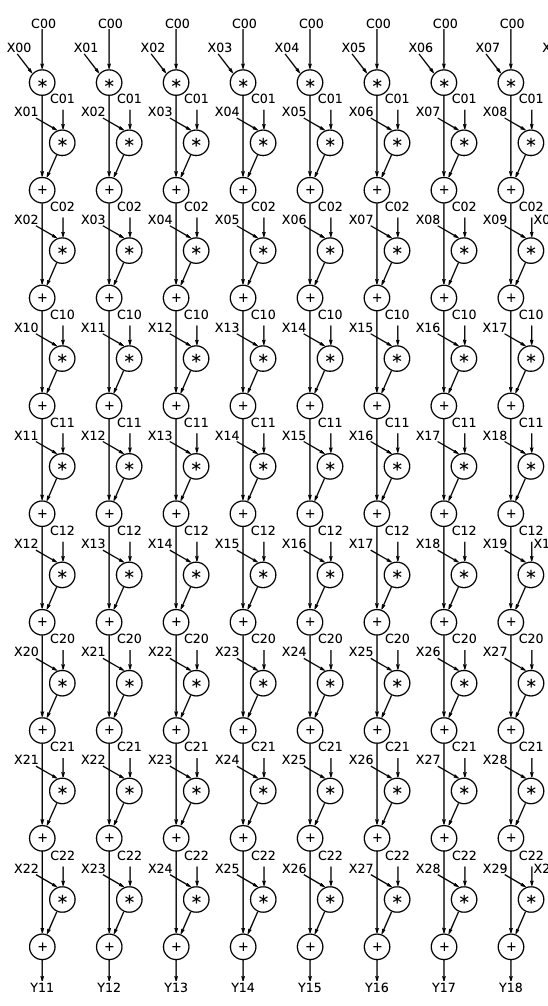
\includegraphics[width=\textwidth,height=6cm,keepaspectratio=true]{../figs/2D_strategy.png}
%    \caption{}
%    \label{}
%\end{figure}
%------------------------------
%% Simple table
%\begin{center}
%\begin{tabular}{ |c|c| } 
% \hline
%
% \hline
%\end{tabular}
%\end{center}

\section{Amdahl's Law(1P)}
1. 
\begin{align*}
  Eff &= \frac{Sp}{p} \\
      &= \frac{1}{sp + (1-s)} \\
      &= \frac{1}{0.1p + 0.9} \geq 0.7
\end{align*}
Solve the inequality above we have $p \leq 5.2$, since $p$ muss be a integer, we have $p_{max} = 5$.
\\
\\
2.
For a given Program, if the non-parallelizable part of a program accounts for 10\% of the runtime (p = 0.9), we can get no more than a 10 times speedup, regardless of how many processors are added. This puts an upper limit on the usefulness of adding more parallel execution units. 
On the other hand, if we want to achieve 70\% efficiency,
There's a upper bound of the number of processes $p$, meaning, the more processes we use, the worse the efficiency becomes.
\\
Amdahl's law only applies to cases where the problem size is fixed. In practice, as more computing resources become available, 
they tend to get used on larger problems (larger datasets), and the time spent in the parallelizable part often grows much faster than the inherently serial work.
In this case, Gustafson's law gives a less pessimistic and more realistic assessment of parallel performance\cite{Gustafson}:
$$
S_{latency}(s)=1-p+sp
$$

\section{Process Pinning within a Compute Node (1P)}
\subsection{Task 1 - 2 MPI and 4 OMP}

\begin{lstlisting}[frame=single]
di29waj@i22r07c05s03:~/hpclab/A3/src/pinning$ OMP_NUM_THREADS=4 \
    I_MPI_PIN_DOMAIN=omp I_MPI_PIN_ORDER=scatter \
    I_MPI_PIN_CELL=core mpirun -np 2 ./pinning
rank=0; thread=0; cpu id=0
rank=0; thread=1; cpu id=1
rank=0; thread=2; cpu id=2
rank=0; thread=3; cpu id=3
rank=1; thread=0; cpu id=14
rank=1; thread=1; cpu id=15
rank=1; thread=2; cpu id=16
rank=1; thread=3; cpu id=17
\end{lstlisting}

\subsection{Task 2 - 4 MPI and 2 OMP}
\begin{lstlisting}[frame=single]
di29waj@i22r07c05s03:~/hpclab/A3/src/pinning$ OMP_NUM_THREADS=2 \
    KMP_AFFINITY="explicit,proclist=[0,6,7,13,14,20,21,27]" \
    I_MPI_PIN_ORDER=spread mpiexec -n 4 ./pinning 2> /dev/null
rank=0; thread=0; cpu id=0
rank=0; thread=1; cpu id=6
rank=1; thread=0; cpu id=7
rank=1; thread=1; cpu id=13
rank=2; thread=0; cpu id=14
rank=2; thread=1; cpu id=20
rank=3; thread=0; cpu id=21
rank=3; thread=1; cpu id=27
\end{lstlisting}

\subsection{Optional task - pinning for a pure MPI job}
When running a job on a cluster, besides pinning MPI processes through environment variables, one can also achieve the same thing though srun variables. For example, to get the same pinning as in the task 1 and task 2, we need the following variables:
\begin{itemize}
  \item -n <number of MPI tasks> 
  \item --mpi=pmi2 : specify which PMI library to use
  \item --cpu-bind=map\_cpu:<list of cores>
  \item --hint=nomultithread: disable hyperthreading
\end{itemize}
The MPI pinning in task 1 and task 2 (without OpenMP) can be acchieved as follows:
\begin{lstlisting}[frame=single]
di29waj@i22r07c05s02:~/hpclab/A3/src/pinning$ srun -n 2 --mpi=pmi2 \
    --cpu-bind=map_cpu:0,14  --hint=nomultithread ./pinning
rank=0; thread=0; cpu id=0
rank=1; thread=0; cpu id=14

di29waj@i22r07c05s02:~/hpclab/A3/src/pinning$ srun -n 4 --mpi=pmi2 \
    --cpu-bind=map_cpu:0,7,14,21  --hint=nomultithread ./pinning
rank=0; thread=0; cpu id=0
rank=1; thread=0; cpu id=7
rank=2; thread=0; cpu id=14
rank=3; thread=0; cpu id=21
\end{lstlisting}

\section{Analyzing an HPC Network (2P)}
\subsection{General information about OmniPath}
Omni-Path Architecture (OPA) is a Intel's high-performance communication architecture which is used for as interconnects for communications in a some supercomputers, for example SuperMUC-NG, CoolMUC-3. The target of Ommin-Path is lower communication latency, lower power consumption, and a higher throughput. It is claimed by Intel as a better alternative to Nvidia's Mellanox Infiniband for communications in big-scale applications. 
The special features of OPA for traffic management refered from \cite{omnipath} are:
\begin{itemize}
  \item Adaptive Routing: selects the least congested path to balance the packet load.
  \item Dispersive Routing: distributes packets across multiple paths to reduce congestion.
  \item Traffic Flow Optimization: diminishes the variation in latency for high priority traffic.
  \item Packet Integrity Protection: allows for rapid, transparent recovery from transmission errors.
\end{itemize}

\paragraph{ Explain why the bandwidth depends on the message size}
According to \cite{Mark16}, the Omni-Path HFI has different hardware support for different send modes which are Programmed I/O (PIO) send and send direct memory access (SDMA). 
The PCI Express (PCIe) of PIO hardware blocks has the bandwidth of 10.6 GBps while the one of SDMA has the bandwidth of 12.5 GBps. The paper also provided the information that the sending small messages usually envolves PIO send contexts, whereas SDMA engines are used for large message transfers.Thus, the bandwidth depends on the message size, the bandwidth is larger when sending big-size messages since SDMA hardware is used for Verbs transaction and SMMA blocks have higher maximum bandwith.

The paper \cite{Taffet19} also measure how the bandwith depends on the message size, as presented below:
\begin{figure}[htpb]
    \centering
    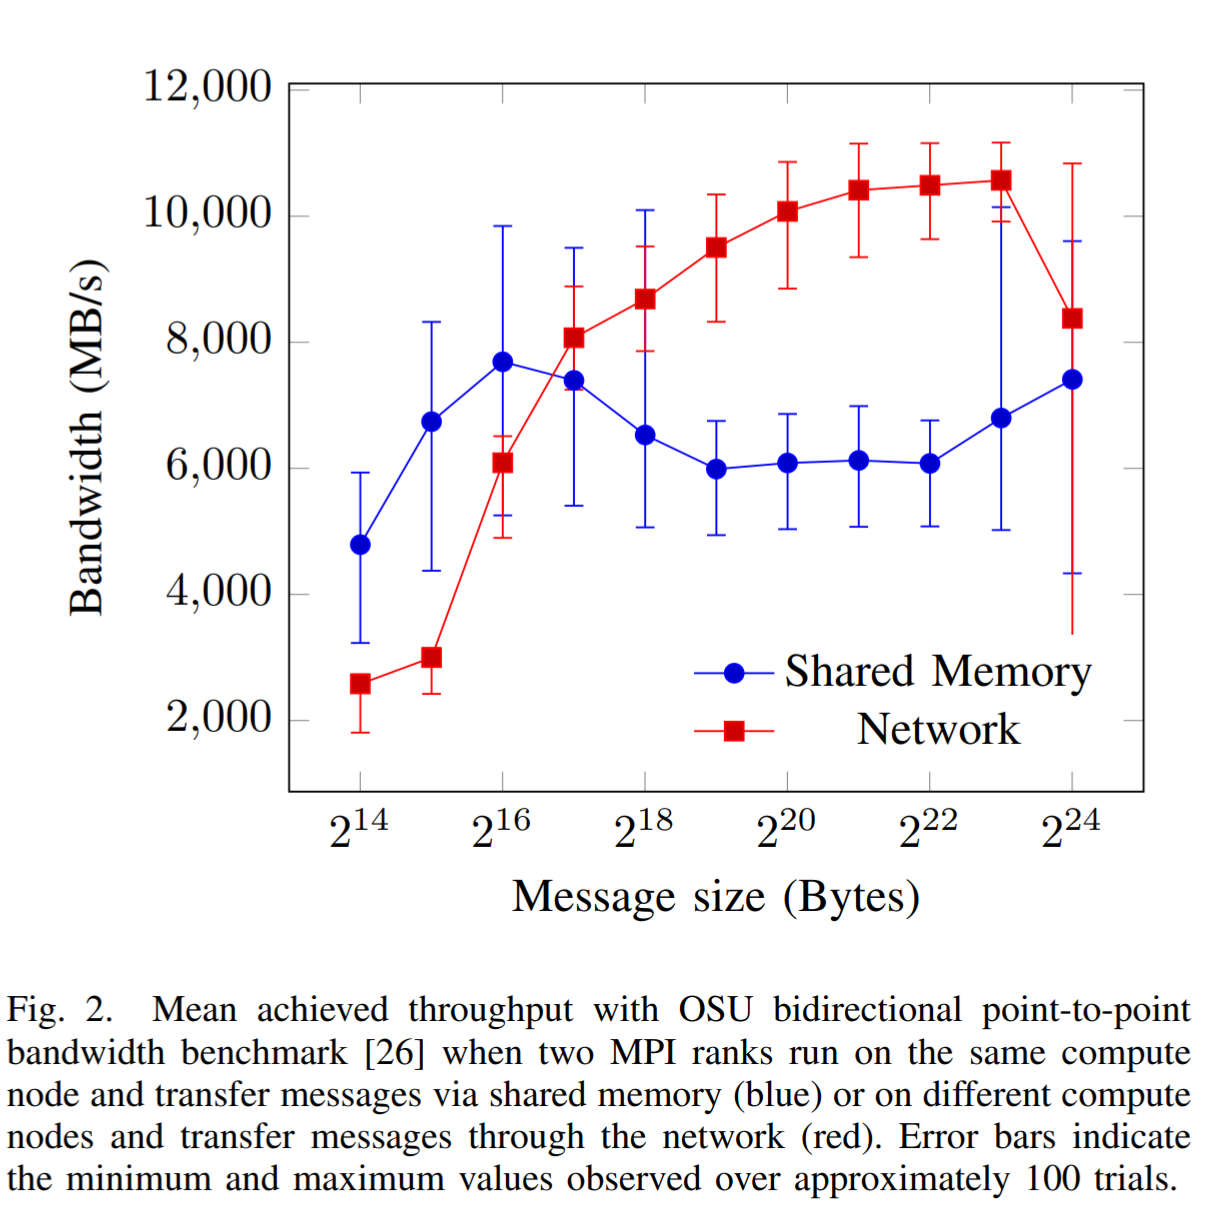
\includegraphics[width=0.75\textwidth,keepaspectratio=true]{../figs/3_bandwith_vs_size.png}
    \caption{Measurement of bandwith respect to message sizes \cite{Taffet19}}
    \label{fig:bandwith1}
\end{figure}
In Fig. \ref{fig:bandwith1}, when transfering messages with size of $2^{14}$, the bandwith is only around 2500 MB/s. The bandwith increases when the transfered-message sizes are increased, reaching the peak of 11000 MB/s at the message size $2^20$. This confirmed out previous explaination.

\paragraph{ What latencies and peak bandwidths can you expect?}
For peak bandwiths, one can expect the maximum bandwith that PCIe of SDMA can handle which is 12.5 GBps. For latency, according to \cite{omnipath}, it can be as small as 1 microsecond for small messages, and up to miliseconds for large messages.

\subsection{Network Topology}
The topology for provided information is presented in the Figure \ref{fig:ntopo}.
\begin{figure}[htpb]
    \centering
    \resizebox{\columnwidth}{!}{
    % Graphic for TeX using PGF
% Title: /home/bichphuong/CSE/WS21/hpclab/A3/report/Network_topology.dia
% Creator: Dia v0.97+git
% CreationDate: Mon Nov 29 16:12:16 2021
% For: bichphuong
% \usepackage{tikz}
% The following commands are not supported in PSTricks at present
% We define them conditionally, so when they are implemented,
% this pgf file will use them.
\ifx\du\undefined
  \newlength{\du}
\fi
\setlength{\du}{15\unitlength}
\begin{tikzpicture}[even odd rule]
\pgftransformxscale{1.000000}
\pgftransformyscale{-1.000000}
\definecolor{dialinecolor}{rgb}{0.000000, 0.000000, 0.000000}
\pgfsetstrokecolor{dialinecolor}
\pgfsetstrokeopacity{1.000000}
\definecolor{diafillcolor}{rgb}{1.000000, 1.000000, 1.000000}
\pgfsetfillcolor{diafillcolor}
\pgfsetfillopacity{1.000000}
\pgfsetlinewidth{0.100000\du}
\pgfsetdash{}{0pt}
\pgfsetbuttcap
{
\definecolor{diafillcolor}{rgb}{0.000000, 0.000000, 0.000000}
\pgfsetfillcolor{diafillcolor}
\pgfsetfillopacity{1.000000}
% was here!!!
\definecolor{dialinecolor}{rgb}{0.000000, 0.000000, 0.000000}
\pgfsetstrokecolor{dialinecolor}
\pgfsetstrokeopacity{1.000000}
\draw (31.497751\du,9.350421\du)--(15.538849\du,13.243399\du);
}
\pgfsetlinewidth{0.100000\du}
\pgfsetdash{}{0pt}
\pgfsetbuttcap
{
\definecolor{diafillcolor}{rgb}{0.000000, 0.000000, 0.000000}
\pgfsetfillcolor{diafillcolor}
\pgfsetfillopacity{1.000000}
% was here!!!
\definecolor{dialinecolor}{rgb}{0.000000, 0.000000, 0.000000}
\pgfsetstrokecolor{dialinecolor}
\pgfsetstrokeopacity{1.000000}
\draw (31.539151\du,9.126001\du)--(15.580349\du,13.018999\du);
}
\pgfsetlinewidth{0.100000\du}
\pgfsetdash{}{0pt}
\pgfsetbuttcap
{
\definecolor{diafillcolor}{rgb}{0.000000, 0.000000, 0.000000}
\pgfsetfillcolor{diafillcolor}
\pgfsetfillopacity{1.000000}
% was here!!!
\definecolor{dialinecolor}{rgb}{0.000000, 0.000000, 0.000000}
\pgfsetstrokecolor{dialinecolor}
\pgfsetstrokeopacity{1.000000}
\draw (23.653370\du,9.416367\du)--(14.940030\du,12.729743\du);
}
\pgfsetlinewidth{0.100000\du}
\pgfsetdash{}{0pt}
\pgfsetbuttcap
{
\definecolor{diafillcolor}{rgb}{0.000000, 0.000000, 0.000000}
\pgfsetfillcolor{diafillcolor}
\pgfsetfillopacity{1.000000}
% was here!!!
\definecolor{dialinecolor}{rgb}{0.000000, 0.000000, 0.000000}
\pgfsetstrokecolor{dialinecolor}
\pgfsetstrokeopacity{1.000000}
\draw (16.654196\du,9.577900\du)--(12.646604\du,13.058750\du);
}
\pgfsetlinewidth{0.100000\du}
\pgfsetdash{}{0pt}
\pgfsetbuttcap
{
\definecolor{diafillcolor}{rgb}{0.000000, 0.000000, 0.000000}
\pgfsetfillcolor{diafillcolor}
\pgfsetfillopacity{1.000000}
% was here!!!
\definecolor{dialinecolor}{rgb}{0.000000, 0.000000, 0.000000}
\pgfsetstrokecolor{dialinecolor}
\pgfsetstrokeopacity{1.000000}
\draw (9.653233\du,9.796662\du)--(10.824497\du,13.193538\du);
}
\pgfsetlinewidth{0.100000\du}
\pgfsetdash{}{0pt}
\pgfsetmiterjoin
{\pgfsetcornersarced{\pgfpoint{0.000000\du}{0.000000\du}}\definecolor{diafillcolor}{rgb}{1.000000, 1.000000, 1.000000}
\pgfsetfillcolor{diafillcolor}
\pgfsetfillopacity{1.000000}
\fill (5.586620\du,11.696900\du)--(5.586620\du,23.271002\du)--(17.257984\du,23.271002\du)--(17.257984\du,11.696900\du)--cycle;
}{\pgfsetcornersarced{\pgfpoint{0.000000\du}{0.000000\du}}\definecolor{dialinecolor}{rgb}{0.000000, 0.000000, 0.000000}
\pgfsetstrokecolor{dialinecolor}
\pgfsetstrokeopacity{1.000000}
\draw (5.586620\du,11.696900\du)--(5.586620\du,23.271002\du)--(17.257984\du,23.271002\du)--(17.257984\du,11.696900\du)--cycle;
}% setfont left to latex
\definecolor{dialinecolor}{rgb}{0.000000, 0.000000, 0.000000}
\pgfsetstrokecolor{dialinecolor}
\pgfsetstrokeopacity{1.000000}
\definecolor{diafillcolor}{rgb}{0.000000, 0.000000, 0.000000}
\pgfsetfillcolor{diafillcolor}
\pgfsetfillopacity{1.000000}
\node[anchor=base,inner sep=0pt, outer sep=0pt,color=dialinecolor] at (11.422302\du,17.678014\du){};
\pgfsetlinewidth{0.100000\du}
\pgfsetdash{}{0pt}
\pgfsetbuttcap
{
\definecolor{diafillcolor}{rgb}{0.000000, 0.000000, 0.000000}
\pgfsetfillcolor{diafillcolor}
\pgfsetfillopacity{1.000000}
% was here!!!
\definecolor{dialinecolor}{rgb}{0.000000, 0.000000, 0.000000}
\pgfsetstrokecolor{dialinecolor}
\pgfsetstrokeopacity{1.000000}
\draw (16.685897\du,9.809141\du)--(12.678303\du,13.289949\du);
}
\pgfsetlinewidth{0.100000\du}
\pgfsetdash{}{0pt}
\pgfsetbuttcap
{
\definecolor{diafillcolor}{rgb}{0.000000, 0.000000, 0.000000}
\pgfsetfillcolor{diafillcolor}
\pgfsetfillopacity{1.000000}
% was here!!!
\definecolor{dialinecolor}{rgb}{0.000000, 0.000000, 0.000000}
\pgfsetstrokecolor{dialinecolor}
\pgfsetstrokeopacity{1.000000}
\draw (10.033902\du,9.943862\du)--(11.205198\du,13.340738\du);
}
\pgfsetlinewidth{0.100000\du}
\pgfsetdash{}{0pt}
\pgfsetmiterjoin
{\pgfsetcornersarced{\pgfpoint{0.000000\du}{0.000000\du}}\definecolor{diafillcolor}{rgb}{1.000000, 1.000000, 1.000000}
\pgfsetfillcolor{diafillcolor}
\pgfsetfillopacity{1.000000}
\fill (6.445250\du,12.183200\du)--(6.445250\du,23.757302\du)--(18.116614\du,23.757302\du)--(18.116614\du,12.183200\du)--cycle;
}{\pgfsetcornersarced{\pgfpoint{0.000000\du}{0.000000\du}}\definecolor{dialinecolor}{rgb}{0.000000, 0.000000, 0.000000}
\pgfsetstrokecolor{dialinecolor}
\pgfsetstrokeopacity{1.000000}
\draw (6.445250\du,12.183200\du)--(6.445250\du,23.757302\du)--(18.116614\du,23.757302\du)--(18.116614\du,12.183200\du)--cycle;
}% setfont left to latex
\definecolor{dialinecolor}{rgb}{0.000000, 0.000000, 0.000000}
\pgfsetstrokecolor{dialinecolor}
\pgfsetstrokeopacity{1.000000}
\definecolor{diafillcolor}{rgb}{0.000000, 0.000000, 0.000000}
\pgfsetfillcolor{diafillcolor}
\pgfsetfillopacity{1.000000}
\node[anchor=base,inner sep=0pt, outer sep=0pt,color=dialinecolor] at (12.280932\du,18.164314\du){};
\pgfsetlinewidth{0.100000\du}
\pgfsetdash{}{0pt}
\pgfsetbuttcap
{
\definecolor{diafillcolor}{rgb}{0.000000, 0.000000, 0.000000}
\pgfsetfillcolor{diafillcolor}
\pgfsetfillopacity{1.000000}
% was here!!!
\definecolor{dialinecolor}{rgb}{0.000000, 0.000000, 0.000000}
\pgfsetstrokecolor{dialinecolor}
\pgfsetstrokeopacity{1.000000}
\draw (23.632270\du,9.647606\du)--(14.919030\du,12.961044\du);
}
\pgfsetlinewidth{0.100000\du}
\pgfsetdash{}{0pt}
\pgfsetmiterjoin
{\pgfsetcornersarced{\pgfpoint{0.000000\du}{0.000000\du}}\definecolor{diafillcolor}{rgb}{1.000000, 1.000000, 1.000000}
\pgfsetfillcolor{diafillcolor}
\pgfsetfillopacity{1.000000}
\fill (27.655000\du,12.831600\du)--(27.655000\du,24.405702\du)--(39.806535\du,24.405702\du)--(39.806535\du,12.831600\du)--cycle;
}{\pgfsetcornersarced{\pgfpoint{0.000000\du}{0.000000\du}}\definecolor{dialinecolor}{rgb}{0.000000, 0.000000, 0.000000}
\pgfsetstrokecolor{dialinecolor}
\pgfsetstrokeopacity{1.000000}
\draw (27.655000\du,12.831600\du)--(27.655000\du,24.405702\du)--(39.806535\du,24.405702\du)--(39.806535\du,12.831600\du)--cycle;
}% setfont left to latex
\definecolor{dialinecolor}{rgb}{0.000000, 0.000000, 0.000000}
\pgfsetstrokecolor{dialinecolor}
\pgfsetstrokeopacity{1.000000}
\definecolor{diafillcolor}{rgb}{0.000000, 0.000000, 0.000000}
\pgfsetfillcolor{diafillcolor}
\pgfsetfillopacity{1.000000}
\node[anchor=base,inner sep=0pt, outer sep=0pt,color=dialinecolor] at (33.730768\du,18.812714\du){};
\pgfsetlinewidth{0.100000\du}
\pgfsetdash{}{0pt}
\pgfsetmiterjoin
{\pgfsetcornersarced{\pgfpoint{0.000000\du}{0.000000\du}}\definecolor{diafillcolor}{rgb}{1.000000, 1.000000, 1.000000}
\pgfsetfillcolor{diafillcolor}
\pgfsetfillopacity{1.000000}
\fill (7.831030\du,12.616500\du)--(7.831030\du,24.190602\du)--(19.502394\du,24.190602\du)--(19.502394\du,12.616500\du)--cycle;
}{\pgfsetcornersarced{\pgfpoint{0.000000\du}{0.000000\du}}\definecolor{dialinecolor}{rgb}{0.000000, 0.000000, 0.000000}
\pgfsetstrokecolor{dialinecolor}
\pgfsetstrokeopacity{1.000000}
\draw (7.831030\du,12.616500\du)--(7.831030\du,24.190602\du)--(19.502394\du,24.190602\du)--(19.502394\du,12.616500\du)--cycle;
}% setfont left to latex
\definecolor{dialinecolor}{rgb}{0.000000, 0.000000, 0.000000}
\pgfsetstrokecolor{dialinecolor}
\pgfsetstrokeopacity{1.000000}
\definecolor{diafillcolor}{rgb}{0.000000, 0.000000, 0.000000}
\pgfsetfillcolor{diafillcolor}
\pgfsetfillopacity{1.000000}
\node[anchor=base,inner sep=0pt, outer sep=0pt,color=dialinecolor] at (13.666712\du,18.597614\du){};
\pgfsetlinewidth{0.100000\du}
\pgfsetdash{}{0pt}
\pgfsetbuttcap
{
\definecolor{diafillcolor}{rgb}{0.000000, 0.000000, 0.000000}
\pgfsetfillcolor{diafillcolor}
\pgfsetfillopacity{1.000000}
% was here!!!
\definecolor{dialinecolor}{rgb}{0.000000, 0.000000, 0.000000}
\pgfsetstrokecolor{dialinecolor}
\pgfsetstrokeopacity{1.000000}
\draw (10.743215\du,10.188868\du)--(11.914435\du,13.585821\du);
}
\pgfsetlinewidth{0.100000\du}
\pgfsetdash{}{0pt}
\pgfsetmiterjoin
{\pgfsetcornersarced{\pgfpoint{0.000000\du}{0.000000\du}}\definecolor{diafillcolor}{rgb}{1.000000, 1.000000, 1.000000}
\pgfsetfillcolor{diafillcolor}
\pgfsetfillopacity{1.000000}
\fill (9.086790\du,19.617200\du)--(9.086790\du,21.567200\du)--(15.386790\du,21.567200\du)--(15.386790\du,19.617200\du)--cycle;
}{\pgfsetcornersarced{\pgfpoint{0.000000\du}{0.000000\du}}\definecolor{dialinecolor}{rgb}{0.000000, 0.000000, 0.000000}
\pgfsetstrokecolor{dialinecolor}
\pgfsetstrokeopacity{1.000000}
\draw (9.086790\du,19.617200\du)--(9.086790\du,21.567200\du)--(15.386790\du,21.567200\du)--(15.386790\du,19.617200\du)--cycle;
}% setfont left to latex
\definecolor{dialinecolor}{rgb}{0.000000, 0.000000, 0.000000}
\pgfsetstrokecolor{dialinecolor}
\pgfsetstrokeopacity{1.000000}
\definecolor{diafillcolor}{rgb}{0.000000, 0.000000, 0.000000}
\pgfsetfillcolor{diafillcolor}
\pgfsetfillopacity{1.000000}
\node[anchor=base,inner sep=0pt, outer sep=0pt,color=dialinecolor] at (12.236790\du,20.786262\du){Compute Node};
\pgfsetlinewidth{0.100000\du}
\pgfsetdash{}{0pt}
\pgfsetbuttcap
{
\definecolor{diafillcolor}{rgb}{0.000000, 0.000000, 0.000000}
\pgfsetfillcolor{diafillcolor}
\pgfsetfillopacity{1.000000}
% was here!!!
\definecolor{dialinecolor}{rgb}{0.000000, 0.000000, 0.000000}
\pgfsetstrokecolor{dialinecolor}
\pgfsetstrokeopacity{1.000000}
\draw (13.713135\du,15.453001\du)--(13.692965\du,20.091399\du);
}
\pgfsetlinewidth{0.100000\du}
\pgfsetdash{}{0pt}
\pgfsetmiterjoin
{\pgfsetcornersarced{\pgfpoint{0.000000\du}{0.000000\du}}\definecolor{diafillcolor}{rgb}{1.000000, 1.000000, 1.000000}
\pgfsetfillcolor{diafillcolor}
\pgfsetfillopacity{1.000000}
\fill (9.460660\du,20.041400\du)--(9.460660\du,21.991400\du)--(15.760660\du,21.991400\du)--(15.760660\du,20.041400\du)--cycle;
}{\pgfsetcornersarced{\pgfpoint{0.000000\du}{0.000000\du}}\definecolor{dialinecolor}{rgb}{0.000000, 0.000000, 0.000000}
\pgfsetstrokecolor{dialinecolor}
\pgfsetstrokeopacity{1.000000}
\draw (9.460660\du,20.041400\du)--(9.460660\du,21.991400\du)--(15.760660\du,21.991400\du)--(15.760660\du,20.041400\du)--cycle;
}% setfont left to latex
\definecolor{dialinecolor}{rgb}{0.000000, 0.000000, 0.000000}
\pgfsetstrokecolor{dialinecolor}
\pgfsetstrokeopacity{1.000000}
\definecolor{diafillcolor}{rgb}{0.000000, 0.000000, 0.000000}
\pgfsetfillcolor{diafillcolor}
\pgfsetfillopacity{1.000000}
\node[anchor=base,inner sep=0pt, outer sep=0pt,color=dialinecolor] at (12.610660\du,21.210462\du){Compute Node};
\pgfsetlinewidth{0.100000\du}
\pgfsetdash{}{0pt}
\pgfsetmiterjoin
{\pgfsetcornersarced{\pgfpoint{0.000000\du}{0.000000\du}}\definecolor{diafillcolor}{rgb}{1.000000, 1.000000, 1.000000}
\pgfsetfillcolor{diafillcolor}
\pgfsetfillopacity{1.000000}
\fill (9.774300\du,20.452600\du)--(9.774300\du,22.402600\du)--(16.074300\du,22.402600\du)--(16.074300\du,20.452600\du)--cycle;
}{\pgfsetcornersarced{\pgfpoint{0.000000\du}{0.000000\du}}\definecolor{dialinecolor}{rgb}{0.000000, 0.000000, 0.000000}
\pgfsetstrokecolor{dialinecolor}
\pgfsetstrokeopacity{1.000000}
\draw (9.774300\du,20.452600\du)--(9.774300\du,22.402600\du)--(16.074300\du,22.402600\du)--(16.074300\du,20.452600\du)--cycle;
}% setfont left to latex
\definecolor{dialinecolor}{rgb}{0.000000, 0.000000, 0.000000}
\pgfsetstrokecolor{dialinecolor}
\pgfsetstrokeopacity{1.000000}
\definecolor{diafillcolor}{rgb}{0.000000, 0.000000, 0.000000}
\pgfsetfillcolor{diafillcolor}
\pgfsetfillopacity{1.000000}
\node[anchor=base,inner sep=0pt, outer sep=0pt,color=dialinecolor] at (12.924300\du,21.621662\du){Compute Node};
\pgfsetlinewidth{0.100000\du}
\pgfsetdash{}{0pt}
\pgfsetbuttcap
{
\definecolor{diafillcolor}{rgb}{0.000000, 0.000000, 0.000000}
\pgfsetfillcolor{diafillcolor}
\pgfsetfillopacity{1.000000}
% was here!!!
\definecolor{dialinecolor}{rgb}{0.000000, 0.000000, 0.000000}
\pgfsetstrokecolor{dialinecolor}
\pgfsetstrokeopacity{1.000000}
\draw (14.460579\du,15.526202\du)--(14.429321\du,20.924298\du);
}
\pgfsetlinewidth{0.100000\du}
\pgfsetdash{}{0pt}
\pgfsetmiterjoin
{\pgfsetcornersarced{\pgfpoint{0.000000\du}{0.000000\du}}\definecolor{diafillcolor}{rgb}{1.000000, 1.000000, 1.000000}
\pgfsetfillcolor{diafillcolor}
\pgfsetfillopacity{1.000000}
\fill (10.195600\du,20.874000\du)--(10.195600\du,22.824000\du)--(16.495600\du,22.824000\du)--(16.495600\du,20.874000\du)--cycle;
}{\pgfsetcornersarced{\pgfpoint{0.000000\du}{0.000000\du}}\definecolor{dialinecolor}{rgb}{0.000000, 0.000000, 0.000000}
\pgfsetstrokecolor{dialinecolor}
\pgfsetstrokeopacity{1.000000}
\draw (10.195600\du,20.874000\du)--(10.195600\du,22.824000\du)--(16.495600\du,22.824000\du)--(16.495600\du,20.874000\du)--cycle;
}% setfont left to latex
\definecolor{dialinecolor}{rgb}{0.000000, 0.000000, 0.000000}
\pgfsetstrokecolor{dialinecolor}
\pgfsetstrokeopacity{1.000000}
\definecolor{diafillcolor}{rgb}{0.000000, 0.000000, 0.000000}
\pgfsetfillcolor{diafillcolor}
\pgfsetfillopacity{1.000000}
\node[anchor=base,inner sep=0pt, outer sep=0pt,color=dialinecolor] at (13.345600\du,22.043062\du){Compute Node};
\pgfsetlinewidth{0.100000\du}
\pgfsetdash{}{0pt}
\pgfsetbuttcap
{
\definecolor{diafillcolor}{rgb}{0.000000, 0.000000, 0.000000}
\pgfsetfillcolor{diafillcolor}
\pgfsetfillopacity{1.000000}
% was here!!!
\definecolor{dialinecolor}{rgb}{0.000000, 0.000000, 0.000000}
\pgfsetstrokecolor{dialinecolor}
\pgfsetstrokeopacity{1.000000}
\draw (12.235544\du,15.441849\du)--(12.236566\du,19.666851\du);
}
\pgfsetlinewidth{0.100000\du}
\pgfsetdash{}{0pt}
\pgfsetbuttcap
{
\definecolor{diafillcolor}{rgb}{0.000000, 0.000000, 0.000000}
\pgfsetfillcolor{diafillcolor}
\pgfsetfillopacity{1.000000}
% was here!!!
\definecolor{dialinecolor}{rgb}{0.000000, 0.000000, 0.000000}
\pgfsetstrokecolor{dialinecolor}
\pgfsetstrokeopacity{1.000000}
\draw (14.048472\du,15.499003\du)--(14.009828\du,20.502297\du);
}
\pgfsetlinewidth{0.100000\du}
\pgfsetdash{}{0pt}
\pgfsetbuttcap
{
\definecolor{diafillcolor}{rgb}{0.000000, 0.000000, 0.000000}
\pgfsetfillcolor{diafillcolor}
\pgfsetfillopacity{1.000000}
% was here!!!
\definecolor{dialinecolor}{rgb}{0.000000, 0.000000, 0.000000}
\pgfsetstrokecolor{dialinecolor}
\pgfsetstrokeopacity{1.000000}
\draw (12.410800\du,17.268400\du)--(12.021900\du,17.583700\du);
}
\pgfsetlinewidth{0.100000\du}
\pgfsetdash{}{0pt}
\pgfsetbuttcap
{
\definecolor{diafillcolor}{rgb}{0.000000, 0.000000, 0.000000}
\pgfsetfillcolor{diafillcolor}
\pgfsetfillopacity{1.000000}
% was here!!!
\definecolor{dialinecolor}{rgb}{0.000000, 0.000000, 0.000000}
\pgfsetstrokecolor{dialinecolor}
\pgfsetstrokeopacity{1.000000}
\draw (13.913500\du,18.070100\du)--(13.524600\du,18.385400\du);
}
\pgfsetlinewidth{0.100000\du}
\pgfsetdash{}{0pt}
\pgfsetbuttcap
{
\definecolor{diafillcolor}{rgb}{0.000000, 0.000000, 0.000000}
\pgfsetfillcolor{diafillcolor}
\pgfsetfillopacity{1.000000}
% was here!!!
\definecolor{dialinecolor}{rgb}{0.000000, 0.000000, 0.000000}
\pgfsetstrokecolor{dialinecolor}
\pgfsetstrokeopacity{1.000000}
\draw (14.281400\du,18.306600\du)--(13.892500\du,18.621900\du);
}
\pgfsetlinewidth{0.100000\du}
\pgfsetdash{}{0pt}
\pgfsetbuttcap
{
\definecolor{diafillcolor}{rgb}{0.000000, 0.000000, 0.000000}
\pgfsetfillcolor{diafillcolor}
\pgfsetfillopacity{1.000000}
% was here!!!
\definecolor{dialinecolor}{rgb}{0.000000, 0.000000, 0.000000}
\pgfsetstrokecolor{dialinecolor}
\pgfsetstrokeopacity{1.000000}
\draw (14.661100\du,18.496200\du)--(14.272100\du,18.811600\du);
}
% setfont left to latex
\definecolor{dialinecolor}{rgb}{0.000000, 0.000000, 0.000000}
\pgfsetstrokecolor{dialinecolor}
\pgfsetstrokeopacity{1.000000}
\definecolor{diafillcolor}{rgb}{0.000000, 0.000000, 0.000000}
\pgfsetfillcolor{diafillcolor}
\pgfsetfillopacity{1.000000}
\node[anchor=base west,inner sep=0pt,outer sep=0pt,color=dialinecolor] at (11.533100\du,17.667800\du){2};
% setfont left to latex
\definecolor{dialinecolor}{rgb}{0.000000, 0.000000, 0.000000}
\pgfsetstrokecolor{dialinecolor}
\pgfsetstrokeopacity{1.000000}
\definecolor{diafillcolor}{rgb}{0.000000, 0.000000, 0.000000}
\pgfsetfillcolor{diafillcolor}
\pgfsetfillopacity{1.000000}
\node[anchor=base west,inner sep=0pt,outer sep=0pt,color=dialinecolor] at (16.832300\du,21.576400\du){x 16};
\pgfsetlinewidth{0.100000\du}
\pgfsetdash{}{0pt}
\pgfsetmiterjoin
{\pgfsetcornersarced{\pgfpoint{0.000000\du}{0.000000\du}}\definecolor{diafillcolor}{rgb}{1.000000, 1.000000, 1.000000}
\pgfsetfillcolor{diafillcolor}
\pgfsetfillopacity{1.000000}
\fill (7.826140\du,8.333740\du)--(7.826140\du,10.233740\du)--(13.036140\du,10.233740\du)--(13.036140\du,8.333740\du)--cycle;
}{\pgfsetcornersarced{\pgfpoint{0.000000\du}{0.000000\du}}\definecolor{dialinecolor}{rgb}{0.000000, 0.000000, 0.000000}
\pgfsetstrokecolor{dialinecolor}
\pgfsetstrokeopacity{1.000000}
\draw (7.826140\du,8.333740\du)--(7.826140\du,10.233740\du)--(13.036140\du,10.233740\du)--(13.036140\du,8.333740\du)--cycle;
}% setfont left to latex
\definecolor{dialinecolor}{rgb}{0.000000, 0.000000, 0.000000}
\pgfsetstrokecolor{dialinecolor}
\pgfsetstrokeopacity{1.000000}
\definecolor{diafillcolor}{rgb}{0.000000, 0.000000, 0.000000}
\pgfsetfillcolor{diafillcolor}
\pgfsetfillopacity{1.000000}
\node[anchor=base,inner sep=0pt, outer sep=0pt,color=dialinecolor] at (10.431140\du,9.477803\du){Spine Switch};
\pgfsetlinewidth{0.100000\du}
\pgfsetdash{}{0pt}
\pgfsetbuttcap
{
\definecolor{diafillcolor}{rgb}{0.000000, 0.000000, 0.000000}
\pgfsetfillcolor{diafillcolor}
\pgfsetfillopacity{1.000000}
% was here!!!
\definecolor{dialinecolor}{rgb}{0.000000, 0.000000, 0.000000}
\pgfsetstrokecolor{dialinecolor}
\pgfsetstrokeopacity{1.000000}
\draw (17.271635\du,10.142118\du)--(13.264022\du,13.623002\du);
}
\pgfsetlinewidth{0.100000\du}
\pgfsetdash{}{0pt}
\pgfsetmiterjoin
{\pgfsetcornersarced{\pgfpoint{0.000000\du}{0.000000\du}}\definecolor{diafillcolor}{rgb}{1.000000, 1.000000, 1.000000}
\pgfsetfillcolor{diafillcolor}
\pgfsetfillopacity{1.000000}
\fill (15.666600\du,8.323580\du)--(15.666600\du,10.223580\du)--(20.876600\du,10.223580\du)--(20.876600\du,8.323580\du)--cycle;
}{\pgfsetcornersarced{\pgfpoint{0.000000\du}{0.000000\du}}\definecolor{dialinecolor}{rgb}{0.000000, 0.000000, 0.000000}
\pgfsetstrokecolor{dialinecolor}
\pgfsetstrokeopacity{1.000000}
\draw (15.666600\du,8.323580\du)--(15.666600\du,10.223580\du)--(20.876600\du,10.223580\du)--(20.876600\du,8.323580\du)--cycle;
}% setfont left to latex
\definecolor{dialinecolor}{rgb}{0.000000, 0.000000, 0.000000}
\pgfsetstrokecolor{dialinecolor}
\pgfsetstrokeopacity{1.000000}
\definecolor{diafillcolor}{rgb}{0.000000, 0.000000, 0.000000}
\pgfsetfillcolor{diafillcolor}
\pgfsetfillopacity{1.000000}
\node[anchor=base,inner sep=0pt, outer sep=0pt,color=dialinecolor] at (18.271600\du,9.467643\du){Spine Switch};
\pgfsetlinewidth{0.100000\du}
\pgfsetdash{}{0pt}
\pgfsetmiterjoin
{\pgfsetcornersarced{\pgfpoint{0.000000\du}{0.000000\du}}\definecolor{diafillcolor}{rgb}{1.000000, 1.000000, 1.000000}
\pgfsetfillcolor{diafillcolor}
\pgfsetfillopacity{1.000000}
\fill (9.085320\du,13.541500\du)--(9.085320\du,15.491500\du)--(15.385320\du,15.491500\du)--(15.385320\du,13.541500\du)--cycle;
}{\pgfsetcornersarced{\pgfpoint{0.000000\du}{0.000000\du}}\definecolor{dialinecolor}{rgb}{0.000000, 0.000000, 0.000000}
\pgfsetstrokecolor{dialinecolor}
\pgfsetstrokeopacity{1.000000}
\draw (9.085320\du,13.541500\du)--(9.085320\du,15.491500\du)--(15.385320\du,15.491500\du)--(15.385320\du,13.541500\du)--cycle;
}% setfont left to latex
\definecolor{dialinecolor}{rgb}{0.000000, 0.000000, 0.000000}
\pgfsetstrokecolor{dialinecolor}
\pgfsetstrokeopacity{1.000000}
\definecolor{diafillcolor}{rgb}{0.000000, 0.000000, 0.000000}
\pgfsetfillcolor{diafillcolor}
\pgfsetfillopacity{1.000000}
\node[anchor=base,inner sep=0pt, outer sep=0pt,color=dialinecolor] at (12.235320\du,14.710562\du){Leaf Switch};
% setfont left to latex
\definecolor{dialinecolor}{rgb}{0.000000, 0.000000, 0.000000}
\pgfsetstrokecolor{dialinecolor}
\pgfsetstrokeopacity{1.000000}
\definecolor{diafillcolor}{rgb}{0.000000, 0.000000, 0.000000}
\pgfsetfillcolor{diafillcolor}
\pgfsetfillopacity{1.000000}
\node[anchor=base west,inner sep=0pt,outer sep=0pt,color=dialinecolor] at (15.899200\du,15.308000\du){32 down};
% setfont left to latex
\definecolor{dialinecolor}{rgb}{0.000000, 0.000000, 0.000000}
\pgfsetstrokecolor{dialinecolor}
\pgfsetstrokeopacity{1.000000}
\definecolor{diafillcolor}{rgb}{0.000000, 0.000000, 0.000000}
\pgfsetfillcolor{diafillcolor}
\pgfsetfillopacity{1.000000}
\node[anchor=base west,inner sep=0pt,outer sep=0pt,color=dialinecolor] at (15.841300\du,14.267000\du){16 up};
% setfont left to latex
\definecolor{dialinecolor}{rgb}{0.000000, 0.000000, 0.000000}
\pgfsetstrokecolor{dialinecolor}
\pgfsetstrokeopacity{1.000000}
\definecolor{diafillcolor}{rgb}{0.000000, 0.000000, 0.000000}
\pgfsetfillcolor{diafillcolor}
\pgfsetfillopacity{1.000000}
\node[anchor=base west,inner sep=0pt,outer sep=0pt,color=dialinecolor] at (12.065900\du,28.285000\du){};
% setfont left to latex
\definecolor{dialinecolor}{rgb}{0.000000, 0.000000, 0.000000}
\pgfsetstrokecolor{dialinecolor}
\pgfsetstrokeopacity{1.000000}
\definecolor{diafillcolor}{rgb}{0.000000, 0.000000, 0.000000}
\pgfsetfillcolor{diafillcolor}
\pgfsetfillopacity{1.000000}
\node[anchor=base west,inner sep=0pt,outer sep=0pt,color=dialinecolor] at (19.736000\du,24.859700\du){x9};
% setfont left to latex
\definecolor{dialinecolor}{rgb}{0.000000, 0.000000, 0.000000}
\pgfsetstrokecolor{dialinecolor}
\pgfsetstrokeopacity{1.000000}
\definecolor{diafillcolor}{rgb}{0.000000, 0.000000, 0.000000}
\pgfsetfillcolor{diafillcolor}
\pgfsetfillopacity{1.000000}
\node[anchor=base west,inner sep=0pt,outer sep=0pt,color=dialinecolor] at (26.554775\du,24.812100\du){x1};
\pgfsetlinewidth{0.100000\du}
\pgfsetdash{}{0pt}
\pgfsetbuttcap
{
\definecolor{diafillcolor}{rgb}{0.000000, 0.000000, 0.000000}
\pgfsetfillcolor{diafillcolor}
\pgfsetfillopacity{1.000000}
% was here!!!
\definecolor{dialinecolor}{rgb}{0.000000, 0.000000, 0.000000}
\pgfsetstrokecolor{dialinecolor}
\pgfsetstrokeopacity{1.000000}
\draw (27.244675\du,10.184976\du)--(31.347971\du,13.491327\du);
}
\pgfsetlinewidth{0.100000\du}
\pgfsetdash{}{0pt}
\pgfsetmiterjoin
{\pgfsetcornersarced{\pgfpoint{0.000000\du}{0.000000\du}}\definecolor{diafillcolor}{rgb}{1.000000, 1.000000, 1.000000}
\pgfsetfillcolor{diafillcolor}
\pgfsetfillopacity{1.000000}
\fill (29.388000\du,19.549800\du)--(29.388000\du,21.499800\du)--(35.688000\du,21.499800\du)--(35.688000\du,19.549800\du)--cycle;
}{\pgfsetcornersarced{\pgfpoint{0.000000\du}{0.000000\du}}\definecolor{dialinecolor}{rgb}{0.000000, 0.000000, 0.000000}
\pgfsetstrokecolor{dialinecolor}
\pgfsetstrokeopacity{1.000000}
\draw (29.388000\du,19.549800\du)--(29.388000\du,21.499800\du)--(35.688000\du,21.499800\du)--(35.688000\du,19.549800\du)--cycle;
}% setfont left to latex
\definecolor{dialinecolor}{rgb}{0.000000, 0.000000, 0.000000}
\pgfsetstrokecolor{dialinecolor}
\pgfsetstrokeopacity{1.000000}
\definecolor{diafillcolor}{rgb}{0.000000, 0.000000, 0.000000}
\pgfsetfillcolor{diafillcolor}
\pgfsetfillopacity{1.000000}
\node[anchor=base,inner sep=0pt, outer sep=0pt,color=dialinecolor] at (32.538000\du,20.718863\du){Compute Node};
\pgfsetlinewidth{0.100000\du}
\pgfsetdash{}{0pt}
\pgfsetbuttcap
{
\definecolor{diafillcolor}{rgb}{0.000000, 0.000000, 0.000000}
\pgfsetfillcolor{diafillcolor}
\pgfsetfillopacity{1.000000}
% was here!!!
\definecolor{dialinecolor}{rgb}{0.000000, 0.000000, 0.000000}
\pgfsetstrokecolor{dialinecolor}
\pgfsetstrokeopacity{1.000000}
\draw (32.918010\du,15.385600\du)--(32.912916\du,20.023946\du);
}
\pgfsetlinewidth{0.100000\du}
\pgfsetdash{}{0pt}
\pgfsetmiterjoin
{\pgfsetcornersarced{\pgfpoint{0.000000\du}{0.000000\du}}\definecolor{diafillcolor}{rgb}{1.000000, 1.000000, 1.000000}
\pgfsetfillcolor{diafillcolor}
\pgfsetfillopacity{1.000000}
\fill (29.761900\du,19.974000\du)--(29.761900\du,21.924000\du)--(36.061900\du,21.924000\du)--(36.061900\du,19.974000\du)--cycle;
}{\pgfsetcornersarced{\pgfpoint{0.000000\du}{0.000000\du}}\definecolor{dialinecolor}{rgb}{0.000000, 0.000000, 0.000000}
\pgfsetstrokecolor{dialinecolor}
\pgfsetstrokeopacity{1.000000}
\draw (29.761900\du,19.974000\du)--(29.761900\du,21.924000\du)--(36.061900\du,21.924000\du)--(36.061900\du,19.974000\du)--cycle;
}% setfont left to latex
\definecolor{dialinecolor}{rgb}{0.000000, 0.000000, 0.000000}
\pgfsetstrokecolor{dialinecolor}
\pgfsetstrokeopacity{1.000000}
\definecolor{diafillcolor}{rgb}{0.000000, 0.000000, 0.000000}
\pgfsetfillcolor{diafillcolor}
\pgfsetfillopacity{1.000000}
\node[anchor=base,inner sep=0pt, outer sep=0pt,color=dialinecolor] at (32.911900\du,21.143062\du){Compute Node};
\pgfsetlinewidth{0.100000\du}
\pgfsetdash{}{0pt}
\pgfsetmiterjoin
{\pgfsetcornersarced{\pgfpoint{0.000000\du}{0.000000\du}}\definecolor{diafillcolor}{rgb}{1.000000, 1.000000, 1.000000}
\pgfsetfillcolor{diafillcolor}
\pgfsetfillopacity{1.000000}
\fill (30.075600\du,20.385200\du)--(30.075600\du,22.335200\du)--(36.375600\du,22.335200\du)--(36.375600\du,20.385200\du)--cycle;
}{\pgfsetcornersarced{\pgfpoint{0.000000\du}{0.000000\du}}\definecolor{dialinecolor}{rgb}{0.000000, 0.000000, 0.000000}
\pgfsetstrokecolor{dialinecolor}
\pgfsetstrokeopacity{1.000000}
\draw (30.075600\du,20.385200\du)--(30.075600\du,22.335200\du)--(36.375600\du,22.335200\du)--(36.375600\du,20.385200\du)--cycle;
}% setfont left to latex
\definecolor{dialinecolor}{rgb}{0.000000, 0.000000, 0.000000}
\pgfsetstrokecolor{dialinecolor}
\pgfsetstrokeopacity{1.000000}
\definecolor{diafillcolor}{rgb}{0.000000, 0.000000, 0.000000}
\pgfsetfillcolor{diafillcolor}
\pgfsetfillopacity{1.000000}
\node[anchor=base,inner sep=0pt, outer sep=0pt,color=dialinecolor] at (33.225600\du,21.554263\du){Compute Node};
\pgfsetlinewidth{0.100000\du}
\pgfsetdash{}{0pt}
\pgfsetbuttcap
{
\definecolor{diafillcolor}{rgb}{0.000000, 0.000000, 0.000000}
\pgfsetfillcolor{diafillcolor}
\pgfsetfillopacity{1.000000}
% was here!!!
\definecolor{dialinecolor}{rgb}{0.000000, 0.000000, 0.000000}
\pgfsetstrokecolor{dialinecolor}
\pgfsetstrokeopacity{1.000000}
\draw (33.665596\du,15.458800\du)--(33.649634\du,20.856873\du);
}
\pgfsetlinewidth{0.100000\du}
\pgfsetdash{}{0pt}
\pgfsetmiterjoin
{\pgfsetcornersarced{\pgfpoint{0.000000\du}{0.000000\du}}\definecolor{diafillcolor}{rgb}{1.000000, 1.000000, 1.000000}
\pgfsetfillcolor{diafillcolor}
\pgfsetfillopacity{1.000000}
\fill (30.496900\du,20.806600\du)--(30.496900\du,22.756600\du)--(36.796900\du,22.756600\du)--(36.796900\du,20.806600\du)--cycle;
}{\pgfsetcornersarced{\pgfpoint{0.000000\du}{0.000000\du}}\definecolor{dialinecolor}{rgb}{0.000000, 0.000000, 0.000000}
\pgfsetstrokecolor{dialinecolor}
\pgfsetstrokeopacity{1.000000}
\draw (30.496900\du,20.806600\du)--(30.496900\du,22.756600\du)--(36.796900\du,22.756600\du)--(36.796900\du,20.806600\du)--cycle;
}% setfont left to latex
\definecolor{dialinecolor}{rgb}{0.000000, 0.000000, 0.000000}
\pgfsetstrokecolor{dialinecolor}
\pgfsetstrokeopacity{1.000000}
\definecolor{diafillcolor}{rgb}{0.000000, 0.000000, 0.000000}
\pgfsetfillcolor{diafillcolor}
\pgfsetfillopacity{1.000000}
\node[anchor=base,inner sep=0pt, outer sep=0pt,color=dialinecolor] at (33.646900\du,21.975662\du){Compute Node};
\pgfsetlinewidth{0.100000\du}
\pgfsetdash{}{0pt}
\pgfsetbuttcap
{
\definecolor{diafillcolor}{rgb}{0.000000, 0.000000, 0.000000}
\pgfsetfillcolor{diafillcolor}
\pgfsetfillopacity{1.000000}
% was here!!!
\definecolor{dialinecolor}{rgb}{0.000000, 0.000000, 0.000000}
\pgfsetstrokecolor{dialinecolor}
\pgfsetstrokeopacity{1.000000}
\draw (32.536813\du,15.374449\du)--(32.537787\du,19.599451\du);
}
\pgfsetlinewidth{0.100000\du}
\pgfsetdash{}{0pt}
\pgfsetbuttcap
{
\definecolor{diafillcolor}{rgb}{0.000000, 0.000000, 0.000000}
\pgfsetfillcolor{diafillcolor}
\pgfsetfillopacity{1.000000}
% was here!!!
\definecolor{dialinecolor}{rgb}{0.000000, 0.000000, 0.000000}
\pgfsetstrokecolor{dialinecolor}
\pgfsetstrokeopacity{1.000000}
\draw (33.253470\du,15.431601\du)--(33.229950\du,20.434929\du);
}
\pgfsetlinewidth{0.100000\du}
\pgfsetdash{}{0pt}
\pgfsetbuttcap
{
\definecolor{diafillcolor}{rgb}{0.000000, 0.000000, 0.000000}
\pgfsetfillcolor{diafillcolor}
\pgfsetfillopacity{1.000000}
% was here!!!
\definecolor{dialinecolor}{rgb}{0.000000, 0.000000, 0.000000}
\pgfsetstrokecolor{dialinecolor}
\pgfsetstrokeopacity{1.000000}
\draw (32.712100\du,17.201000\du)--(32.323200\du,17.516300\du);
}
\pgfsetlinewidth{0.100000\du}
\pgfsetdash{}{0pt}
\pgfsetbuttcap
{
\definecolor{diafillcolor}{rgb}{0.000000, 0.000000, 0.000000}
\pgfsetfillcolor{diafillcolor}
\pgfsetfillopacity{1.000000}
% was here!!!
\definecolor{dialinecolor}{rgb}{0.000000, 0.000000, 0.000000}
\pgfsetstrokecolor{dialinecolor}
\pgfsetstrokeopacity{1.000000}
\draw (33.118700\du,17.465200\du)--(32.729800\du,17.780600\du);
}
\pgfsetlinewidth{0.100000\du}
\pgfsetdash{}{0pt}
\pgfsetbuttcap
{
\definecolor{diafillcolor}{rgb}{0.000000, 0.000000, 0.000000}
\pgfsetfillcolor{diafillcolor}
\pgfsetfillopacity{1.000000}
% was here!!!
\definecolor{dialinecolor}{rgb}{0.000000, 0.000000, 0.000000}
\pgfsetstrokecolor{dialinecolor}
\pgfsetstrokeopacity{1.000000}
\draw (33.486600\du,17.701700\du)--(33.097700\du,18.017100\du);
}
\pgfsetlinewidth{0.100000\du}
\pgfsetdash{}{0pt}
\pgfsetbuttcap
{
\definecolor{diafillcolor}{rgb}{0.000000, 0.000000, 0.000000}
\pgfsetfillcolor{diafillcolor}
\pgfsetfillopacity{1.000000}
% was here!!!
\definecolor{dialinecolor}{rgb}{0.000000, 0.000000, 0.000000}
\pgfsetstrokecolor{dialinecolor}
\pgfsetstrokeopacity{1.000000}
\draw (33.891300\du,18.053800\du)--(33.502400\du,18.369200\du);
}
% setfont left to latex
\definecolor{dialinecolor}{rgb}{0.000000, 0.000000, 0.000000}
\pgfsetstrokecolor{dialinecolor}
\pgfsetstrokeopacity{1.000000}
\definecolor{diafillcolor}{rgb}{0.000000, 0.000000, 0.000000}
\pgfsetfillcolor{diafillcolor}
\pgfsetfillopacity{1.000000}
\node[anchor=base west,inner sep=0pt,outer sep=0pt,color=dialinecolor] at (31.834400\du,17.600400\du){2};
\pgfsetlinewidth{0.100000\du}
\pgfsetdash{}{0pt}
\pgfsetbuttcap
{
\definecolor{diafillcolor}{rgb}{0.000000, 0.000000, 0.000000}
\pgfsetfillcolor{diafillcolor}
\pgfsetfillopacity{1.000000}
% was here!!!
\definecolor{dialinecolor}{rgb}{0.000000, 0.000000, 0.000000}
\pgfsetstrokecolor{dialinecolor}
\pgfsetstrokeopacity{1.000000}
\draw (33.645306\du,10.049658\du)--(32.745999\du,13.618187\du);
}
\pgfsetlinewidth{0.100000\du}
\pgfsetdash{}{0pt}
\pgfsetmiterjoin
{\pgfsetcornersarced{\pgfpoint{0.000000\du}{0.000000\du}}\definecolor{diafillcolor}{rgb}{1.000000, 1.000000, 1.000000}
\pgfsetfillcolor{diafillcolor}
\pgfsetfillopacity{1.000000}
\fill (31.243300\du,8.294160\du)--(31.243300\du,10.194160\du)--(36.453300\du,10.194160\du)--(36.453300\du,8.294160\du)--cycle;
}{\pgfsetcornersarced{\pgfpoint{0.000000\du}{0.000000\du}}\definecolor{dialinecolor}{rgb}{0.000000, 0.000000, 0.000000}
\pgfsetstrokecolor{dialinecolor}
\pgfsetstrokeopacity{1.000000}
\draw (31.243300\du,8.294160\du)--(31.243300\du,10.194160\du)--(36.453300\du,10.194160\du)--(36.453300\du,8.294160\du)--cycle;
}% setfont left to latex
\definecolor{dialinecolor}{rgb}{0.000000, 0.000000, 0.000000}
\pgfsetstrokecolor{dialinecolor}
\pgfsetstrokeopacity{1.000000}
\definecolor{diafillcolor}{rgb}{0.000000, 0.000000, 0.000000}
\pgfsetfillcolor{diafillcolor}
\pgfsetfillopacity{1.000000}
\node[anchor=base,inner sep=0pt, outer sep=0pt,color=dialinecolor] at (33.848300\du,9.438223\du){Spine Switch};
\pgfsetlinewidth{0.100000\du}
\pgfsetdash{}{0pt}
\pgfsetmiterjoin
{\pgfsetcornersarced{\pgfpoint{0.000000\du}{0.000000\du}}\definecolor{diafillcolor}{rgb}{1.000000, 1.000000, 1.000000}
\pgfsetfillcolor{diafillcolor}
\pgfsetfillopacity{1.000000}
\fill (29.386600\du,13.474100\du)--(29.386600\du,15.424100\du)--(35.686600\du,15.424100\du)--(35.686600\du,13.474100\du)--cycle;
}{\pgfsetcornersarced{\pgfpoint{0.000000\du}{0.000000\du}}\definecolor{dialinecolor}{rgb}{0.000000, 0.000000, 0.000000}
\pgfsetstrokecolor{dialinecolor}
\pgfsetstrokeopacity{1.000000}
\draw (29.386600\du,13.474100\du)--(29.386600\du,15.424100\du)--(35.686600\du,15.424100\du)--(35.686600\du,13.474100\du)--cycle;
}% setfont left to latex
\definecolor{dialinecolor}{rgb}{0.000000, 0.000000, 0.000000}
\pgfsetstrokecolor{dialinecolor}
\pgfsetstrokeopacity{1.000000}
\definecolor{diafillcolor}{rgb}{0.000000, 0.000000, 0.000000}
\pgfsetfillcolor{diafillcolor}
\pgfsetfillopacity{1.000000}
\node[anchor=base,inner sep=0pt, outer sep=0pt,color=dialinecolor] at (32.536600\du,14.643162\du){Leaf Switch};
% setfont left to latex
\definecolor{dialinecolor}{rgb}{0.000000, 0.000000, 0.000000}
\pgfsetstrokecolor{dialinecolor}
\pgfsetstrokeopacity{1.000000}
\definecolor{diafillcolor}{rgb}{0.000000, 0.000000, 0.000000}
\pgfsetfillcolor{diafillcolor}
\pgfsetfillopacity{1.000000}
\node[anchor=base west,inner sep=0pt,outer sep=0pt,color=dialinecolor] at (35.856343\du,14.036025\du){16 up};
% setfont left to latex
\definecolor{dialinecolor}{rgb}{0.000000, 0.000000, 0.000000}
\pgfsetstrokecolor{dialinecolor}
\pgfsetstrokeopacity{1.000000}
\definecolor{diafillcolor}{rgb}{0.000000, 0.000000, 0.000000}
\pgfsetfillcolor{diafillcolor}
\pgfsetfillopacity{1.000000}
\node[anchor=base west,inner sep=0pt,outer sep=0pt,color=dialinecolor] at (37.252400\du,21.748300\du){x 4};
% setfont left to latex
\definecolor{dialinecolor}{rgb}{0.000000, 0.000000, 0.000000}
\pgfsetstrokecolor{dialinecolor}
\pgfsetstrokeopacity{1.000000}
\definecolor{diafillcolor}{rgb}{0.000000, 0.000000, 0.000000}
\pgfsetfillcolor{diafillcolor}
\pgfsetfillopacity{1.000000}
\node[anchor=base west,inner sep=0pt,outer sep=0pt,color=dialinecolor] at (36.265450\du,14.738743\du){8 down};
\pgfsetlinewidth{0.100000\du}
\pgfsetdash{{\pgflinewidth}{0.200000\du}}{0cm}
\pgfsetbuttcap
{
\definecolor{diafillcolor}{rgb}{0.000000, 0.000000, 0.000000}
\pgfsetfillcolor{diafillcolor}
\pgfsetfillopacity{1.000000}
% was here!!!
\definecolor{dialinecolor}{rgb}{0.000000, 0.000000, 0.000000}
\pgfsetstrokecolor{dialinecolor}
\pgfsetstrokeopacity{1.000000}
\draw (12.521700\du,17.697300\du)--(13.440900\du,18.121500\du);
}
% setfont left to latex
\definecolor{dialinecolor}{rgb}{0.000000, 0.000000, 0.000000}
\pgfsetstrokecolor{dialinecolor}
\pgfsetstrokeopacity{1.000000}
\definecolor{diafillcolor}{rgb}{0.000000, 0.000000, 0.000000}
\pgfsetfillcolor{diafillcolor}
\pgfsetfillopacity{1.000000}
\node[anchor=base west,inner sep=0pt,outer sep=0pt,color=dialinecolor] at (15.417400\du,18.459400\du){};
\pgfsetlinewidth{0.100000\du}
\pgfsetdash{}{0pt}
\pgfsetbuttcap
{
\definecolor{diafillcolor}{rgb}{0.000000, 0.000000, 0.000000}
\pgfsetfillcolor{diafillcolor}
\pgfsetfillopacity{1.000000}
% was here!!!
\definecolor{dialinecolor}{rgb}{0.000000, 0.000000, 0.000000}
\pgfsetstrokecolor{dialinecolor}
\pgfsetstrokeopacity{1.000000}
\draw (23.550737\du,10.213537\du)--(14.837451\du,13.526976\du);
}
\pgfsetlinewidth{0.100000\du}
\pgfsetdash{}{0pt}
\pgfsetbuttcap
{
\definecolor{diafillcolor}{rgb}{0.000000, 0.000000, 0.000000}
\pgfsetfillcolor{diafillcolor}
\pgfsetfillopacity{1.000000}
% was here!!!
\definecolor{dialinecolor}{rgb}{0.000000, 0.000000, 0.000000}
\pgfsetstrokecolor{dialinecolor}
\pgfsetstrokeopacity{1.000000}
\draw (31.290659\du,9.868079\du)--(15.337112\du,13.759839\du);
}
\pgfsetlinewidth{0.100000\du}
\pgfsetdash{}{0pt}
\pgfsetmiterjoin
{\pgfsetcornersarced{\pgfpoint{0.000000\du}{0.000000\du}}\definecolor{diafillcolor}{rgb}{1.000000, 1.000000, 1.000000}
\pgfsetfillcolor{diafillcolor}
\pgfsetfillopacity{1.000000}
\fill (23.479400\du,8.300050\du)--(23.479400\du,10.200050\du)--(28.689400\du,10.200050\du)--(28.689400\du,8.300050\du)--cycle;
}{\pgfsetcornersarced{\pgfpoint{0.000000\du}{0.000000\du}}\definecolor{dialinecolor}{rgb}{0.000000, 0.000000, 0.000000}
\pgfsetstrokecolor{dialinecolor}
\pgfsetstrokeopacity{1.000000}
\draw (23.479400\du,8.300050\du)--(23.479400\du,10.200050\du)--(28.689400\du,10.200050\du)--(28.689400\du,8.300050\du)--cycle;
}% setfont left to latex
\definecolor{dialinecolor}{rgb}{0.000000, 0.000000, 0.000000}
\pgfsetstrokecolor{dialinecolor}
\pgfsetstrokeopacity{1.000000}
\definecolor{diafillcolor}{rgb}{0.000000, 0.000000, 0.000000}
\pgfsetfillcolor{diafillcolor}
\pgfsetfillopacity{1.000000}
\node[anchor=base,inner sep=0pt, outer sep=0pt,color=dialinecolor] at (26.084400\du,9.444113\du){Spine Switch};
\pgfsetlinewidth{0.100000\du}
\pgfsetdash{}{0pt}
\pgfsetbuttcap
{
\definecolor{diafillcolor}{rgb}{0.000000, 0.000000, 0.000000}
\pgfsetfillcolor{diafillcolor}
\pgfsetfillopacity{1.000000}
% was here!!!
\definecolor{dialinecolor}{rgb}{0.000000, 0.000000, 0.000000}
\pgfsetstrokecolor{dialinecolor}
\pgfsetstrokeopacity{1.000000}
\draw (20.832258\du,10.202619\du)--(29.805291\du,13.458147\du);
}
\pgfsetlinewidth{0.100000\du}
\pgfsetdash{}{0pt}
\pgfsetbuttcap
{
\definecolor{diafillcolor}{rgb}{0.000000, 0.000000, 0.000000}
\pgfsetfillcolor{diafillcolor}
\pgfsetfillopacity{1.000000}
% was here!!!
\definecolor{dialinecolor}{rgb}{0.000000, 0.000000, 0.000000}
\pgfsetstrokecolor{dialinecolor}
\pgfsetstrokeopacity{1.000000}
\draw (12.978215\du,9.878912\du)--(29.436349\du,13.724667\du);
}
\pgfsetlinewidth{0.100000\du}
\pgfsetdash{{\pgflinewidth}{0.100000\du}}{0cm}
\pgfsetbuttcap
{
\definecolor{diafillcolor}{rgb}{0.000000, 0.000000, 0.000000}
\pgfsetfillcolor{diafillcolor}
\pgfsetfillopacity{1.000000}
% was here!!!
\definecolor{dialinecolor}{rgb}{0.000000, 0.000000, 0.000000}
\pgfsetstrokecolor{dialinecolor}
\pgfsetstrokeopacity{1.000000}
\draw (10.568000\du,11.006200\du)--(10.942900\du,11.006200\du);
}
\pgfsetlinewidth{0.100000\du}
\pgfsetdash{{\pgflinewidth}{0.100000\du}}{0cm}
\pgfsetbuttcap
{
\definecolor{diafillcolor}{rgb}{0.000000, 0.000000, 0.000000}
\pgfsetfillcolor{diafillcolor}
\pgfsetfillopacity{1.000000}
% was here!!!
\definecolor{dialinecolor}{rgb}{0.000000, 0.000000, 0.000000}
\pgfsetstrokecolor{dialinecolor}
\pgfsetstrokeopacity{1.000000}
\draw (15.551600\du,11.032400\du)--(15.851500\du,11.291400\du);
}
\pgfsetlinewidth{0.100000\du}
\pgfsetdash{{\pgflinewidth}{0.100000\du}}{0cm}
\pgfsetbuttcap
{
\definecolor{diafillcolor}{rgb}{0.000000, 0.000000, 0.000000}
\pgfsetfillcolor{diafillcolor}
\pgfsetfillopacity{1.000000}
% was here!!!
\definecolor{dialinecolor}{rgb}{0.000000, 0.000000, 0.000000}
\pgfsetstrokecolor{dialinecolor}
\pgfsetstrokeopacity{1.000000}
\draw (20.893200\du,10.803600\du)--(21.017600\du,11.093700\du);
}
\pgfsetlinewidth{0.100000\du}
\pgfsetdash{{\pgflinewidth}{0.100000\du}}{0cm}
\pgfsetbuttcap
{
\definecolor{diafillcolor}{rgb}{0.000000, 0.000000, 0.000000}
\pgfsetfillcolor{diafillcolor}
\pgfsetfillopacity{1.000000}
% was here!!!
\definecolor{dialinecolor}{rgb}{0.000000, 0.000000, 0.000000}
\pgfsetstrokecolor{dialinecolor}
\pgfsetstrokeopacity{1.000000}
\draw (22.823700\du,11.550400\du)--(22.885100\du,11.843400\du);
}
\pgfsetlinewidth{0.100000\du}
\pgfsetdash{}{0pt}
\pgfsetbuttcap
{
\definecolor{diafillcolor}{rgb}{0.000000, 0.000000, 0.000000}
\pgfsetfillcolor{diafillcolor}
\pgfsetfillopacity{1.000000}
% was here!!!
\definecolor{dialinecolor}{rgb}{0.000000, 0.000000, 0.000000}
\pgfsetstrokecolor{dialinecolor}
\pgfsetstrokeopacity{1.000000}
\draw (10.146900\du,10.746200\du)--(9.917680\du,11.078600\du);
}
\pgfsetlinewidth{0.100000\du}
\pgfsetdash{}{0pt}
\pgfsetbuttcap
{
\definecolor{diafillcolor}{rgb}{0.000000, 0.000000, 0.000000}
\pgfsetfillcolor{diafillcolor}
\pgfsetfillopacity{1.000000}
% was here!!!
\definecolor{dialinecolor}{rgb}{0.000000, 0.000000, 0.000000}
\pgfsetstrokecolor{dialinecolor}
\pgfsetstrokeopacity{1.000000}
\draw (10.468600\du,10.688500\du)--(10.239400\du,11.020900\du);
}
\pgfsetlinewidth{0.100000\du}
\pgfsetdash{}{0pt}
\pgfsetbuttcap
{
\definecolor{diafillcolor}{rgb}{0.000000, 0.000000, 0.000000}
\pgfsetfillcolor{diafillcolor}
\pgfsetfillopacity{1.000000}
% was here!!!
\definecolor{dialinecolor}{rgb}{0.000000, 0.000000, 0.000000}
\pgfsetstrokecolor{dialinecolor}
\pgfsetstrokeopacity{1.000000}
\draw (11.063900\du,10.608600\du)--(10.812500\du,10.906200\du);
}
% setfont left to latex
\definecolor{dialinecolor}{rgb}{0.000000, 0.000000, 0.000000}
\pgfsetstrokecolor{dialinecolor}
\pgfsetstrokeopacity{1.000000}
\definecolor{diafillcolor}{rgb}{0.000000, 0.000000, 0.000000}
\pgfsetfillcolor{diafillcolor}
\pgfsetfillopacity{1.000000}
\node[anchor=base west,inner sep=0pt,outer sep=0pt,color=dialinecolor] at (9.401890\du,11.181700\du){4};
% setfont left to latex
\definecolor{dialinecolor}{rgb}{0.000000, 0.000000, 0.000000}
\pgfsetstrokecolor{dialinecolor}
\pgfsetstrokeopacity{1.000000}
\definecolor{diafillcolor}{rgb}{0.000000, 0.000000, 0.000000}
\pgfsetfillcolor{diafillcolor}
\pgfsetfillopacity{1.000000}
\node[anchor=base west,inner sep=0pt,outer sep=0pt,color=dialinecolor] at (14.404700\du,11.089600\du){4};
% setfont left to latex
\definecolor{dialinecolor}{rgb}{0.000000, 0.000000, 0.000000}
\pgfsetstrokecolor{dialinecolor}
\pgfsetstrokeopacity{1.000000}
\definecolor{diafillcolor}{rgb}{0.000000, 0.000000, 0.000000}
\pgfsetfillcolor{diafillcolor}
\pgfsetfillopacity{1.000000}
\node[anchor=base west,inner sep=0pt,outer sep=0pt,color=dialinecolor] at (19.373100\du,10.806500\du){4};
% setfont left to latex
\definecolor{dialinecolor}{rgb}{0.000000, 0.000000, 0.000000}
\pgfsetstrokecolor{dialinecolor}
\pgfsetstrokeopacity{1.000000}
\definecolor{diafillcolor}{rgb}{0.000000, 0.000000, 0.000000}
\pgfsetfillcolor{diafillcolor}
\pgfsetfillopacity{1.000000}
\node[anchor=base west,inner sep=0pt,outer sep=0pt,color=dialinecolor] at (24.936800\du,13.482000\du){4};
% setfont left to latex
\definecolor{dialinecolor}{rgb}{0.000000, 0.000000, 0.000000}
\pgfsetstrokecolor{dialinecolor}
\pgfsetstrokeopacity{1.000000}
\definecolor{diafillcolor}{rgb}{0.000000, 0.000000, 0.000000}
\pgfsetfillcolor{diafillcolor}
\pgfsetfillopacity{1.000000}
\node[anchor=base west,inner sep=0pt,outer sep=0pt,color=dialinecolor] at (33.824300\du,11.911600\du){4};
\pgfsetlinewidth{0.100000\du}
\pgfsetdash{}{0pt}
\pgfsetbuttcap
{
\definecolor{diafillcolor}{rgb}{0.000000, 0.000000, 0.000000}
\pgfsetfillcolor{diafillcolor}
\pgfsetfillopacity{1.000000}
% was here!!!
\definecolor{dialinecolor}{rgb}{0.000000, 0.000000, 0.000000}
\pgfsetstrokecolor{dialinecolor}
\pgfsetstrokeopacity{1.000000}
\draw (15.217100\du,10.964200\du)--(14.970300\du,10.883400\du);
}
\pgfsetlinewidth{0.100000\du}
\pgfsetdash{}{0pt}
\pgfsetbuttcap
{
\definecolor{diafillcolor}{rgb}{0.000000, 0.000000, 0.000000}
\pgfsetfillcolor{diafillcolor}
\pgfsetfillopacity{1.000000}
% was here!!!
\definecolor{dialinecolor}{rgb}{0.000000, 0.000000, 0.000000}
\pgfsetstrokecolor{dialinecolor}
\pgfsetstrokeopacity{1.000000}
\draw (15.315900\du,11.153200\du)--(15.047200\du,11.087100\du);
}
\pgfsetlinewidth{0.100000\du}
\pgfsetdash{}{0pt}
\pgfsetbuttcap
{
\definecolor{diafillcolor}{rgb}{0.000000, 0.000000, 0.000000}
\pgfsetfillcolor{diafillcolor}
\pgfsetfillopacity{1.000000}
% was here!!!
\definecolor{dialinecolor}{rgb}{0.000000, 0.000000, 0.000000}
\pgfsetstrokecolor{dialinecolor}
\pgfsetstrokeopacity{1.000000}
\draw (15.927600\du,11.472600\du)--(15.658800\du,11.406600\du);
}
\pgfsetlinewidth{0.100000\du}
\pgfsetdash{}{0pt}
\pgfsetbuttcap
{
\definecolor{diafillcolor}{rgb}{0.000000, 0.000000, 0.000000}
\pgfsetfillcolor{diafillcolor}
\pgfsetfillopacity{1.000000}
% was here!!!
\definecolor{dialinecolor}{rgb}{0.000000, 0.000000, 0.000000}
\pgfsetstrokecolor{dialinecolor}
\pgfsetstrokeopacity{1.000000}
\draw (20.042300\du,10.892800\du)--(19.851600\du,10.749800\du);
}
\pgfsetlinewidth{0.100000\du}
\pgfsetdash{}{0pt}
\pgfsetbuttcap
{
\definecolor{diafillcolor}{rgb}{0.000000, 0.000000, 0.000000}
\pgfsetfillcolor{diafillcolor}
\pgfsetfillopacity{1.000000}
% was here!!!
\definecolor{dialinecolor}{rgb}{0.000000, 0.000000, 0.000000}
\pgfsetstrokecolor{dialinecolor}
\pgfsetstrokeopacity{1.000000}
\draw (20.331500\du,11.004000\du)--(20.140700\du,10.861100\du);
}
\pgfsetlinewidth{0.100000\du}
\pgfsetdash{}{0pt}
\pgfsetbuttcap
{
\definecolor{diafillcolor}{rgb}{0.000000, 0.000000, 0.000000}
\pgfsetfillcolor{diafillcolor}
\pgfsetfillopacity{1.000000}
% was here!!!
\definecolor{dialinecolor}{rgb}{0.000000, 0.000000, 0.000000}
\pgfsetstrokecolor{dialinecolor}
\pgfsetstrokeopacity{1.000000}
\draw (20.765100\du,11.380900\du)--(20.574300\du,11.237900\du);
}
\pgfsetlinewidth{0.100000\du}
\pgfsetdash{}{0pt}
\pgfsetbuttcap
{
\definecolor{diafillcolor}{rgb}{0.000000, 0.000000, 0.000000}
\pgfsetfillcolor{diafillcolor}
\pgfsetfillopacity{1.000000}
% was here!!!
\definecolor{dialinecolor}{rgb}{0.000000, 0.000000, 0.000000}
\pgfsetstrokecolor{dialinecolor}
\pgfsetstrokeopacity{1.000000}
\draw (25.153200\du,12.561100\du)--(25.228200\du,12.874600\du);
}
\pgfsetlinewidth{0.100000\du}
\pgfsetdash{}{0pt}
\pgfsetbuttcap
{
\definecolor{diafillcolor}{rgb}{0.000000, 0.000000, 0.000000}
\pgfsetfillcolor{diafillcolor}
\pgfsetfillopacity{1.000000}
% was here!!!
\definecolor{dialinecolor}{rgb}{0.000000, 0.000000, 0.000000}
\pgfsetstrokecolor{dialinecolor}
\pgfsetstrokeopacity{1.000000}
\draw (25.909800\du,11.900000\du)--(25.854100\du,12.191300\du);
}
\pgfsetlinewidth{0.100000\du}
\pgfsetdash{}{0pt}
\pgfsetbuttcap
{
\definecolor{diafillcolor}{rgb}{0.000000, 0.000000, 0.000000}
\pgfsetfillcolor{diafillcolor}
\pgfsetfillopacity{1.000000}
% was here!!!
\definecolor{dialinecolor}{rgb}{0.000000, 0.000000, 0.000000}
\pgfsetstrokecolor{dialinecolor}
\pgfsetstrokeopacity{1.000000}
\draw (28.765400\du,11.184400\du)--(28.639900\du,11.465300\du);
}
\pgfsetlinewidth{0.100000\du}
\pgfsetdash{}{0pt}
\pgfsetbuttcap
{
\definecolor{diafillcolor}{rgb}{0.000000, 0.000000, 0.000000}
\pgfsetfillcolor{diafillcolor}
\pgfsetfillopacity{1.000000}
% was here!!!
\definecolor{dialinecolor}{rgb}{0.000000, 0.000000, 0.000000}
\pgfsetstrokecolor{dialinecolor}
\pgfsetstrokeopacity{1.000000}
\draw (33.391200\du,11.593600\du)--(33.122700\du,11.694200\du);
}
% setfont left to latex
\definecolor{dialinecolor}{rgb}{0.000000, 0.000000, 0.000000}
\pgfsetstrokecolor{dialinecolor}
\pgfsetstrokeopacity{1.000000}
\definecolor{diafillcolor}{rgb}{0.000000, 0.000000, 0.000000}
\pgfsetfillcolor{diafillcolor}
\pgfsetfillopacity{1.000000}
\node[anchor=base west,inner sep=0pt,outer sep=0pt,color=dialinecolor] at (26.487700\du,11.992300\du){4};
% setfont left to latex
\definecolor{dialinecolor}{rgb}{0.000000, 0.000000, 0.000000}
\pgfsetstrokecolor{dialinecolor}
\pgfsetstrokeopacity{1.000000}
\definecolor{diafillcolor}{rgb}{0.000000, 0.000000, 0.000000}
\pgfsetfillcolor{diafillcolor}
\pgfsetfillopacity{1.000000}
\node[anchor=base west,inner sep=0pt,outer sep=0pt,color=dialinecolor] at (29.243300\du,11.308300\du){4};
\pgfsetlinewidth{0.100000\du}
\pgfsetdash{}{0pt}
\pgfsetbuttcap
{
\definecolor{diafillcolor}{rgb}{0.000000, 0.000000, 0.000000}
\pgfsetfillcolor{diafillcolor}
\pgfsetfillopacity{1.000000}
% was here!!!
\definecolor{dialinecolor}{rgb}{0.000000, 0.000000, 0.000000}
\pgfsetstrokecolor{dialinecolor}
\pgfsetstrokeopacity{1.000000}
\draw (22.098100\du,11.507600\du)--(21.907300\du,11.364700\du);
}
\pgfsetlinewidth{0.100000\du}
\pgfsetdash{}{0pt}
\pgfsetbuttcap
{
\definecolor{diafillcolor}{rgb}{0.000000, 0.000000, 0.000000}
\pgfsetfillcolor{diafillcolor}
\pgfsetfillopacity{1.000000}
% was here!!!
\definecolor{dialinecolor}{rgb}{0.000000, 0.000000, 0.000000}
\pgfsetstrokecolor{dialinecolor}
\pgfsetstrokeopacity{1.000000}
\draw (22.367500\du,11.670600\du)--(22.176700\du,11.527600\du);
}
\pgfsetlinewidth{0.100000\du}
\pgfsetdash{}{0pt}
\pgfsetbuttcap
{
\definecolor{diafillcolor}{rgb}{0.000000, 0.000000, 0.000000}
\pgfsetfillcolor{diafillcolor}
\pgfsetfillopacity{1.000000}
% was here!!!
\definecolor{dialinecolor}{rgb}{0.000000, 0.000000, 0.000000}
\pgfsetstrokecolor{dialinecolor}
\pgfsetstrokeopacity{1.000000}
\draw (22.753700\du,12.048900\du)--(22.563000\du,11.906000\du);
}
% setfont left to latex
\definecolor{dialinecolor}{rgb}{0.000000, 0.000000, 0.000000}
\pgfsetstrokecolor{dialinecolor}
\pgfsetstrokeopacity{1.000000}
\definecolor{diafillcolor}{rgb}{0.000000, 0.000000, 0.000000}
\pgfsetfillcolor{diafillcolor}
\pgfsetfillopacity{1.000000}
\node[anchor=base west,inner sep=0pt,outer sep=0pt,color=dialinecolor] at (35.848893\du,15.374406\du){24 disabled};
% setfont left to latex
\definecolor{dialinecolor}{rgb}{0.000000, 0.000000, 0.000000}
\pgfsetstrokecolor{dialinecolor}
\pgfsetstrokeopacity{1.000000}
\definecolor{diafillcolor}{rgb}{0.000000, 0.000000, 0.000000}
\pgfsetfillcolor{diafillcolor}
\pgfsetfillopacity{1.000000}
\node[anchor=base west,inner sep=0pt,outer sep=0pt,color=dialinecolor] at (37.789106\du,9.366707\du){};
% setfont left to latex
\definecolor{dialinecolor}{rgb}{0.000000, 0.000000, 0.000000}
\pgfsetstrokecolor{dialinecolor}
\pgfsetstrokeopacity{1.000000}
\definecolor{diafillcolor}{rgb}{0.000000, 0.000000, 0.000000}
\pgfsetfillcolor{diafillcolor}
\pgfsetfillopacity{1.000000}
\node[anchor=base west,inner sep=0pt,outer sep=0pt,color=dialinecolor] at (36.679520\du,9.131988\du){40 down};
% setfont left to latex
\definecolor{dialinecolor}{rgb}{0.000000, 0.000000, 0.000000}
\pgfsetstrokecolor{dialinecolor}
\pgfsetstrokeopacity{1.000000}
\definecolor{diafillcolor}{rgb}{0.000000, 0.000000, 0.000000}
\pgfsetfillcolor{diafillcolor}
\pgfsetfillopacity{1.000000}
\node[anchor=base west,inner sep=0pt,outer sep=0pt,color=dialinecolor] at (37.047564\du,10.031653\du){8 disabled};
\end{tikzpicture}

  }
    \caption{Network topology for CoolMUC-3}
    \label{fig:ntopo}
\end{figure}
Since we have 10 leaf switches, each switch have 32 ports for connecting to nodes, and each node has 2 links to fabric, thus we can connect each leaf switch to 16 nodes. With 148 nodes, we can have 9 leaf switches which have 16 nodes/switch, and 1 leaf switch which has 4 nodes/switch (total node = 9*16 + 1*4 = 148 nodes).
Each leaf switch, besides 32 ports for nodes, has 16 ports for the spine switches. Each leaf switch connects to 4 spine switches, thus using 4 ports/spine switch. The ratio of ports for lower level and upper level is 32:16 thus 2:1. 
For the spine switches, each of them connects to 10 leaf switches, so using 4*10 = 40 ports. Thus, there are still 8 unused ports. The information about how spine switches are connected are not provided in the description, thus it is not clear enough for us to illustrate it in the figure.
\subsection{Bisection width and bisection bandwith}
\paragraph{32 nodes} Since we have 10 nodes per leaf switch, then 32 nodes are connected to two leaf switches. Each leaf switch connect to 4 spine switchs with 4 links per spine switch. Thus bisection width is 4*4 = 16 links which is 16 links * 100 Gbit/link = 16000 Gbit.
\paragraph{16 nodes} All nodes are connected to a single switch. Since we don't know how they are routed inside the switch, we assumed 2 following cases:
\begin{itemize}
  \item Assume that all nodes are connected by a single point inside the switch, then the bisection width is the number of links of 8 nodes which is 8*2 = 16 links. The bisection bandwith is then 16000 Gbit.
  \item Assume that all nodes are connected pairwise inside the switch. Then we have $C^{16}_{2}$ connections between nodes. To separate these nodes to 2 domains, one needs to cut $C^{16}_{2} - 2*C^{8}_{2} = 64 $ connections. If each connection is a single link, then the bisection width is 64 whereas the bisection bandwith is 64000 Gbits. If each connection is a double link (the same bandwith as the bandwith between nodes and the leaf switch), then the bisection width is 64*2=128, while the bisection bandwith is 128000 Gbits.
\end{itemize}
\section{Broadcast (3P)}
\subsection{Code}
Trivial Version(root sends messages to all other processes):
\begin{lstlisting}[frame=single]
void my_bcast(void *data, int count, MPI_Datatype datatype, int root,
              MPI_Comm communicator)
{
  int world_rank;
  MPI_Comm_rank(communicator, &world_rank);
  int world_size;
  MPI_Comm_size(communicator, &world_size);

  if (world_rank == root)
  {
    int i;
    for (i = 0; i < world_size; i++)
    {
      if (i != world_rank)
      {
        //root sends message to all other processes
        MPI_Send(data, count, datatype, i, 0, communicator);
      }
    }
  }
  else
  {
    MPI_Recv(data, count, datatype, root, 0, communicator,
    MPI_STATUS_IGNORE);
  }
}
\end{lstlisting}
Tree Topology:
\begin{lstlisting}[frame=single]
void broadcast_tree(void *data, int count, MPI_Datatype datatype, 
                    int root_proc, int end_proc, MPI_Comm communicator)
  {
    if (root_proc == end_proc)
    {
        return;
    }
    int rank;
    MPI_Comm_rank(MPI_COMM_WORLD, &rank);
    int recieve_proc = root_proc + (end_proc - root_proc + 1) / 2;
    if (rank == root_proc)
    {
       MPI_Send(data, count, datatype, recieve_proc, 0, communicator);
    }
    else if (rank == recieve_proc)
    {
        MPI_Recv(data, count, datatype, root_proc, 0, communicator, 
                MPI_STATUS_IGNORE);
    }
    broadcast_tree(data, count, datatype, 
                  root_proc, recieve_proc - 1, communicator);
    broadcast_tree(data, count, datatype, 
                  recieve_proc, end_proc, communicator);
  }
\end{lstlisting}
Buffer Optimization:
\begin{lstlisting}[frame=single]
void broadcast_buffer(void *data, int count, MPI_Datatype datatype, int root,
                      MPI_Comm communicator)
{
    int world_rank;
    MPI_Comm_rank(communicator, &world_rank);
    int world_size;
    MPI_Comm_size(communicator, &world_size);

    int buffer_size = 262144;
    int packet_num = (count / buffer_size); 
    int remainder = count % buffer_size;
    if (world_rank == root)
    {
        for (size_t j = 0; j < packet_num; j++)
        {
            MPI_Send((double *)data + (j * buffer_size), buffer_size, 
            datatype, (world_rank + 1) % world_size, 0, communicator);
        }
        //remainder
        MPI_Send((double *)data + (packet_num*buffer_size), remainder, 
        datatype, (world_rank + 1) % world_size, 0, communicator);
    }
    else
    {
        for (size_t j = 0; j < packet_num; j++)
        {
            MPI_Recv((double *)data + (j * buffer_size), buffer_size, 
            datatype, (world_rank +world_size - 1)% world_size, 0, 
            communicator, MPI_STATUS_IGNORE);
            MPI_Send((double *)data + (j * buffer_size), buffer_size, 
            datatype, (world_rank + 1) % world_size, 0, communicator);
        }
        //remainder
        MPI_Recv((double *)data + (packet_num * buffer_size), remainder, 
        datatype, (world_rank +world_size - 1)% world_size, 0, 
        communicator, MPI_STATUS_IGNORE);
        MPI_Send((double *)data + (packet_num * buffer_size), remainder, 
        datatype, (world_rank + 1) % world_size, 0, communicator);
    }
}
  \end{lstlisting}

\subsection{Evaluation}
1) Optimize the bandwidth\\
From the table \ref{tab::broadcast}, we see that the communication volume w.r.t. message size of the entire broadcast routine 
of trivial and tree are actually the same (in the assignment it's indicated that the communication volume of tree algorithm should be higher than trivial algorithm which really confusing me) 
while the message transformed in critical path of tree algorithm is much less than in trivial algorithm($ \log_2^n$ vs. $n$).
This can also observed from the execution time. Also we see that when the process number is 8, the execution time of MPI\_Bcast is almost the same as 
in trivial algorithm, but as the process number increases, the performance of MPI\_Bcast becomes better than tree algorithm.
This may means, MPI\_Bcast has different algorithm implemented regarding to different process number.
\begin{table}[h!]
  \centering
\begin{tabular}{ |p{2cm}|p{2cm}|p{2cm}|p{3cm}|p{3cm}|p{3cm}|  }
  \hline
   & & \multicolumn{2}{|c|}{Critical Path}& Entire Broadcast &Execution Time \\
  \hline
  Topology & NUM\_PROC & MPI-Msg & Amount of Data & Msg-Size& \\
  \hline
  Trivial & 8 & 7 & $7*16KB$ & $7*16KB$ & 4.67928e-05 \\
    & 14 &13 & $13*16KB$ & $13*16KB$ &  6.7117e-05\\
   & 28 & 27 & $27*16KB$ & $27*16KB$ &  0.000120425\\
   \hline
   Tree & 8 & 3 & $3*16KB$ & $7*16KB$ & 2.04132e-05 \\
   & 14 &4 & $4*16KB$ & $15*16KB$ &  1.99638e-05\\
  & 28 & 5 & $5*16KB$ & $27*16KB$ &  3.4531e-05\\
  \hline
  Buffer & 8 & 7 & $7*16KB$ & $7*16KB$ & 8.91956e-06 \\
  & 14 &13 & $13*16KB$ & $13*16KB$ &  5.6849e-05\\
 & 28 & 27 & $27*16KB$ & $27*16KB$ &  7.08333e-05\\
  \hline
  MPI\_Bcast & 8 & Unknown & Unknown & Unknown & 6.53468e-05 \\
  & 14 & &  &  &  9.25825e-06\\
 & 28 & &  &  &  1.41854e-05\\
  \hline
  \end{tabular}
  \caption{Broadcast using 3 different topology with array size n = 2048}
  \label{tab::broadcast}
\end{table}

\begin{figure}[ht]
  \begin{subfigure}
    \centering
    % include first image
    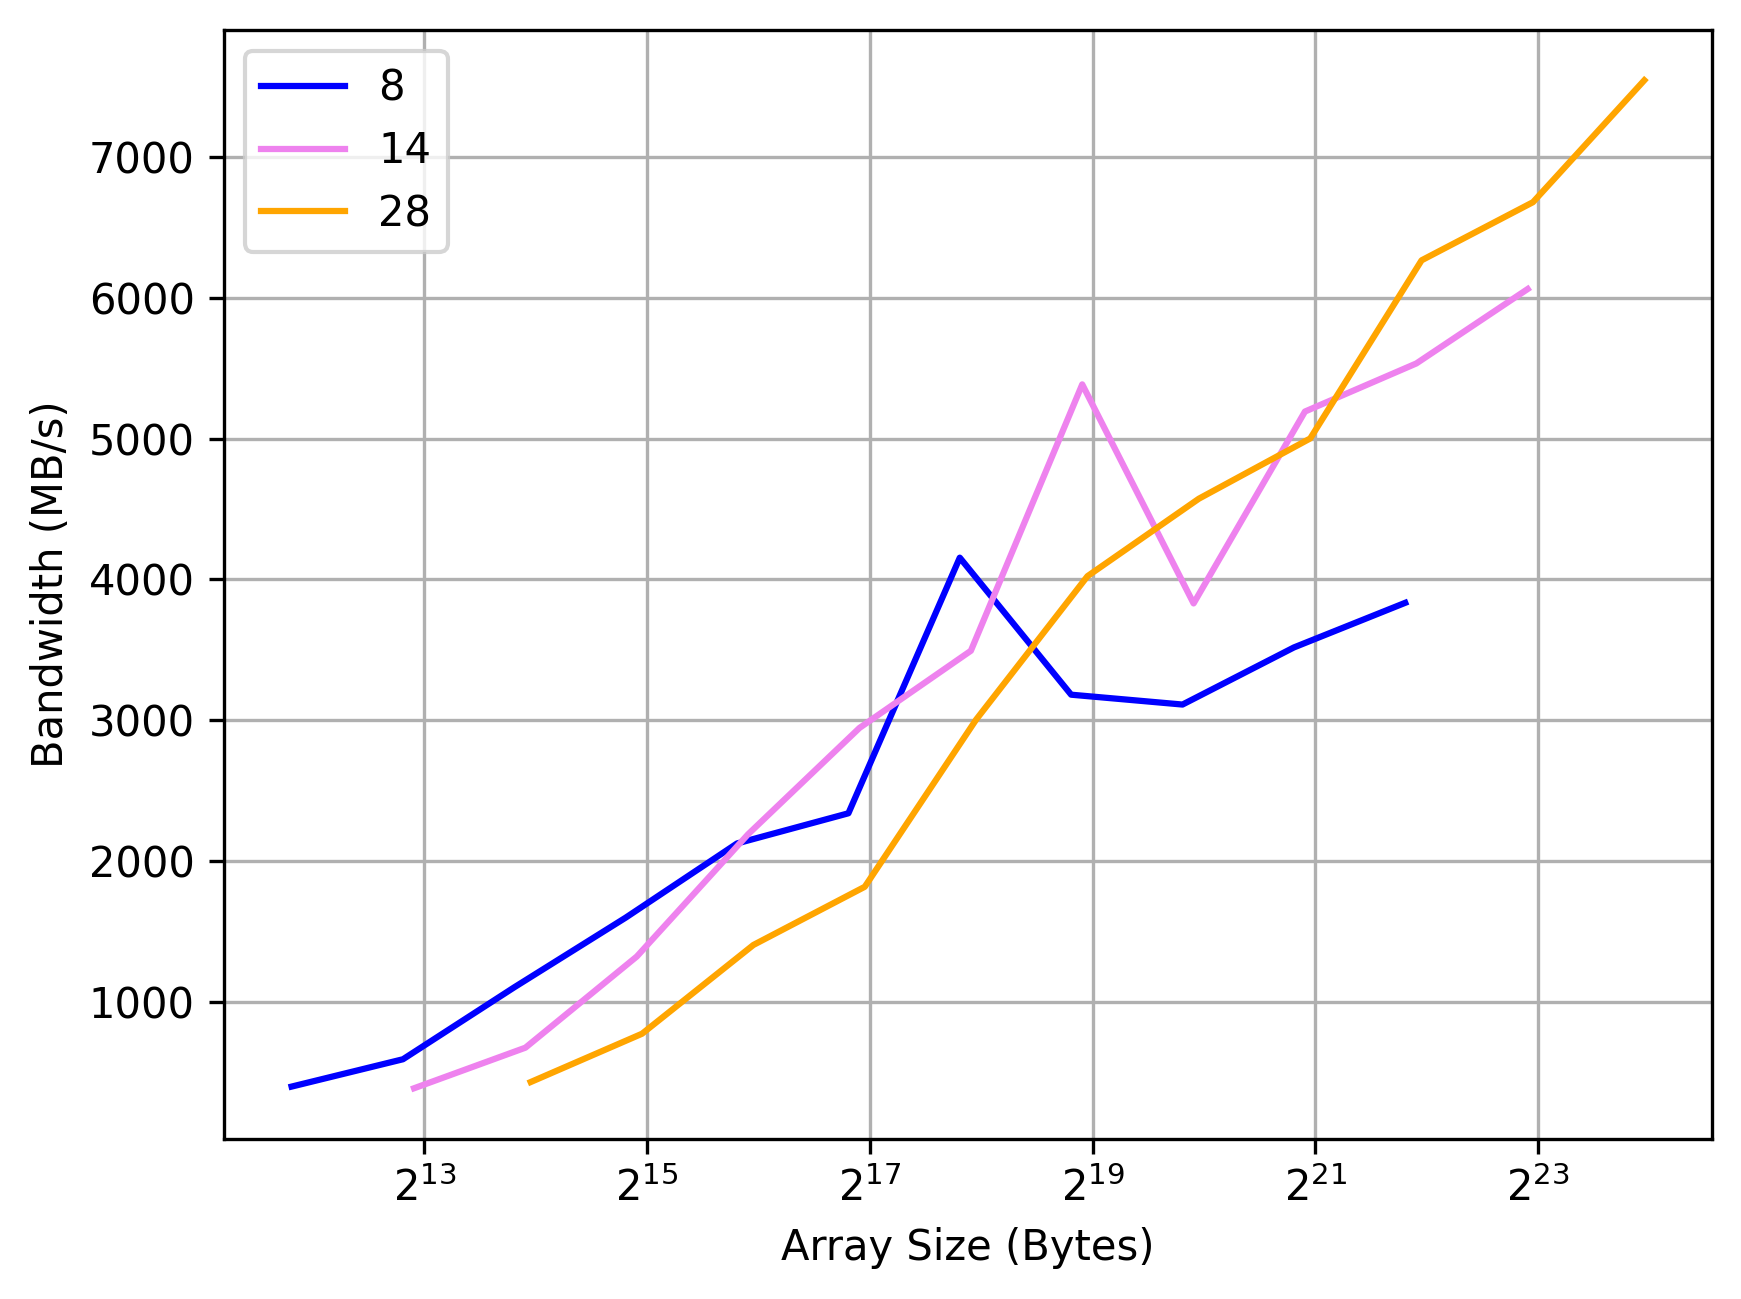
\includegraphics[width=.5\linewidth]{../figs/CollectiveBandwidthTrivial.png}  
  \end{subfigure}
  \begin{subfigure}
    \centering
    % include second image
    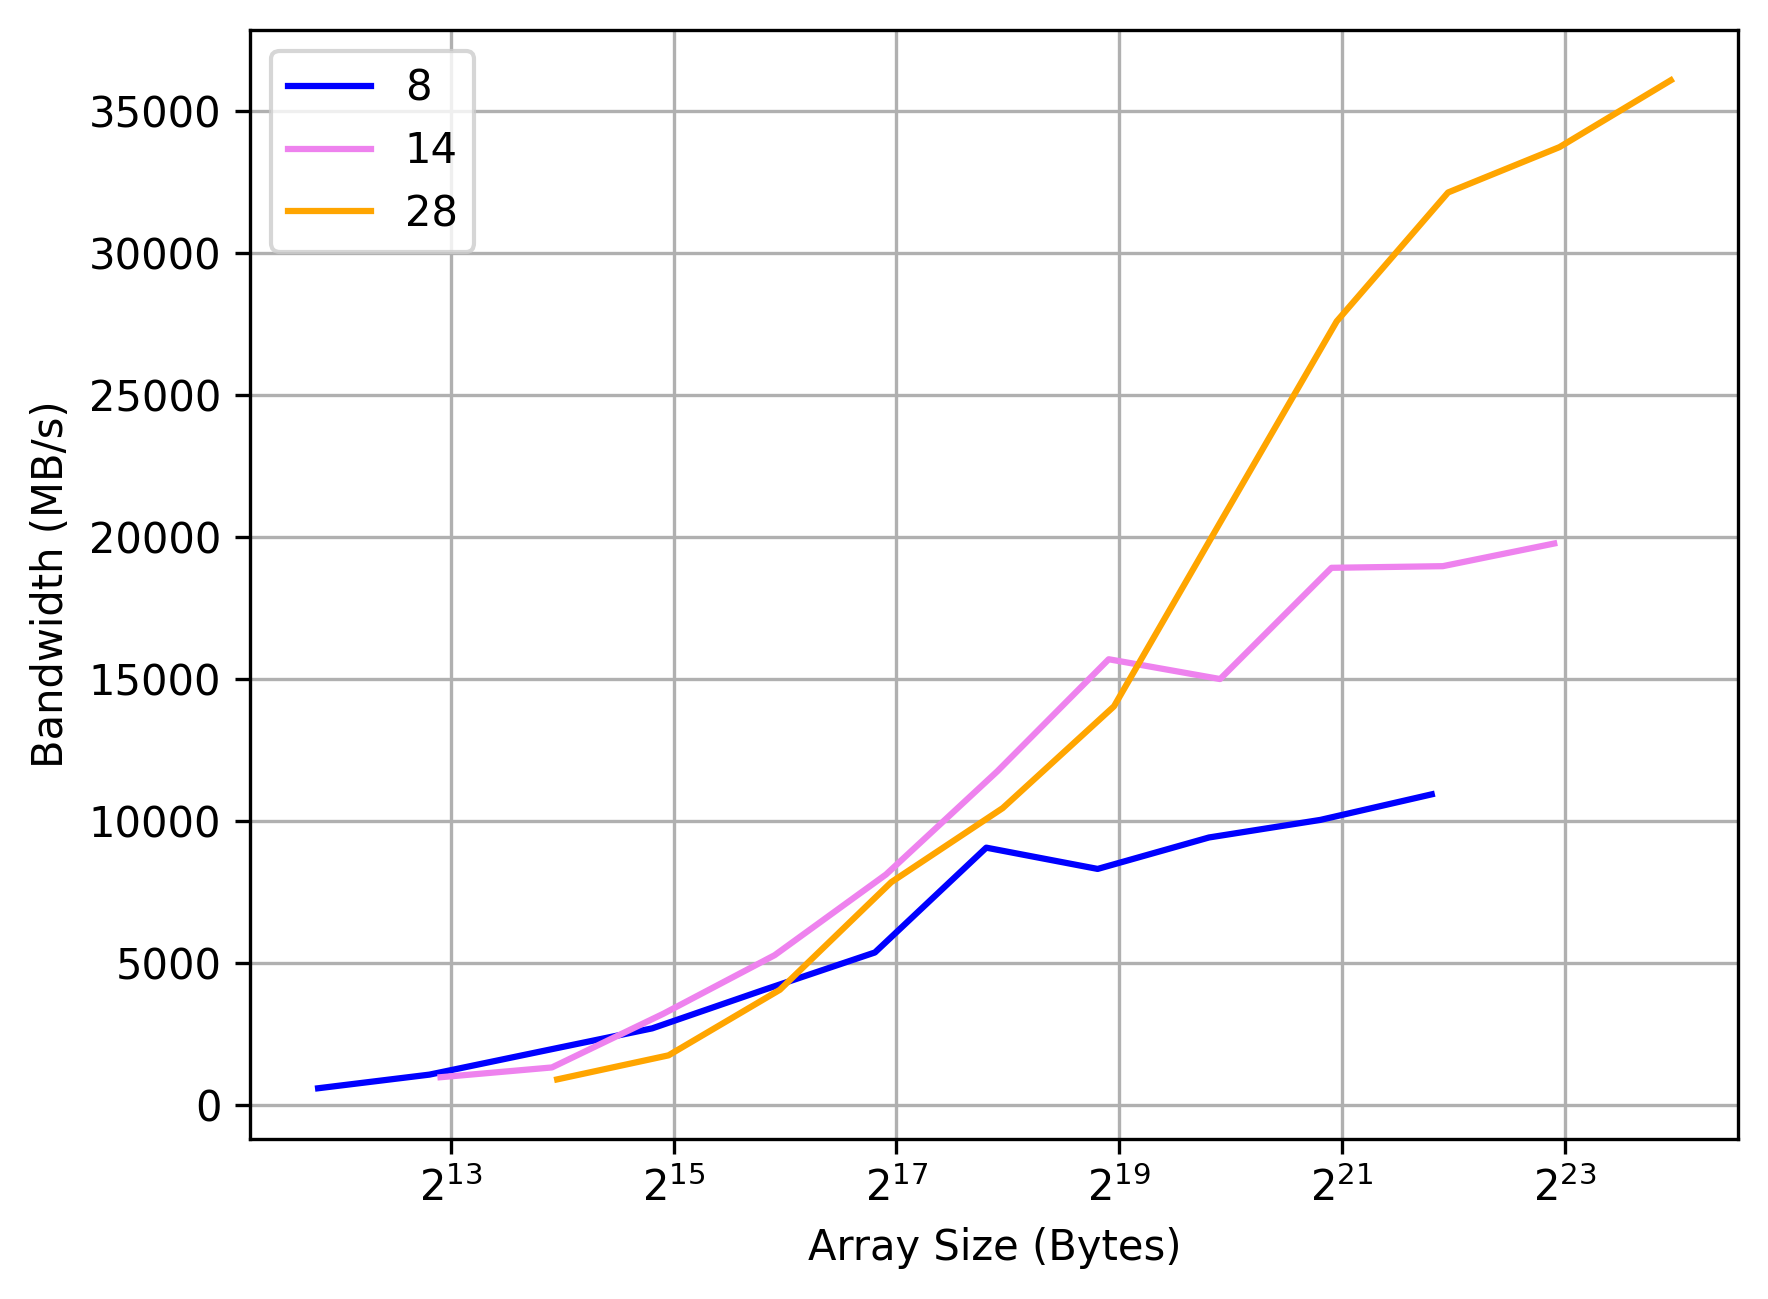
\includegraphics[width=.5\linewidth]{../figs/CollectiveBandwidthTree.png}  
  \end{subfigure}
  \caption{Collective Network Bandwidth (left: Trivial, right: Tree)}
  \label{fig:CNB}
\end{figure}
Figure \ref{fig:CNB} shows the collective network bandwidth of trivial and tree algorithm. 
I expected it to converge when the data size grows(means the channels are fully used). And it seems like not the case in the figure. I am not sure if it's because the data size we choose didn't reach the upper bound of the bandwidth or some other reason.
Also it's notable that there's a big  drop of process 8 and 14. The reason of this could be that MPI uses different protocols regarding to different data size.
There are two protocols of MPI\_Send and Recieve:
\begin{itemize}
  \item Eager protocal
  \subitem Send messages directly, suitable for short messages
  \item Rendezvous protocol
  \subitem Send header to retrive address, then send message, suitable for long messages
\end{itemize}
So instead of sending message directly, rendezvous protocol wait until the receiver told sender the address where he should write the date to,
and this will result in extra time cost and thus reduces the bandwidth.\\
2) Optimize the buffer \\
The idea of optimizing the buffer usage is that when the size of data go beyond the buffer size, we may need to transmit multiple times for one message. While rank 0 is 
transmitting data to rank 1, rank 1 need to wait until all messages are received and then start transmitting to next rank. But this don't have to be like this. We can split the data into multiple small packets,
After rank 1 has received the first packet, it then start to transmit the packet to next rank while still waiting for the second packet from rank 0. The process can be seen below in \ref{fig:buffer}.
Instead of transmitting $(p-1) * (n/buffer\_size)$ packets in critical path, now we only need to transmit $(n/buffer\_size) + p - 2$ packets. One problem remained is how to set the buffer size since 
there is no documentation about the buffer size of MPI(or there is but we can't find), but according to our observation above, we decide to choose the buffer size where the bandwidth drops, so $n = 2^{18}$. \\
\begin{figure}[htpb]
  \centering
  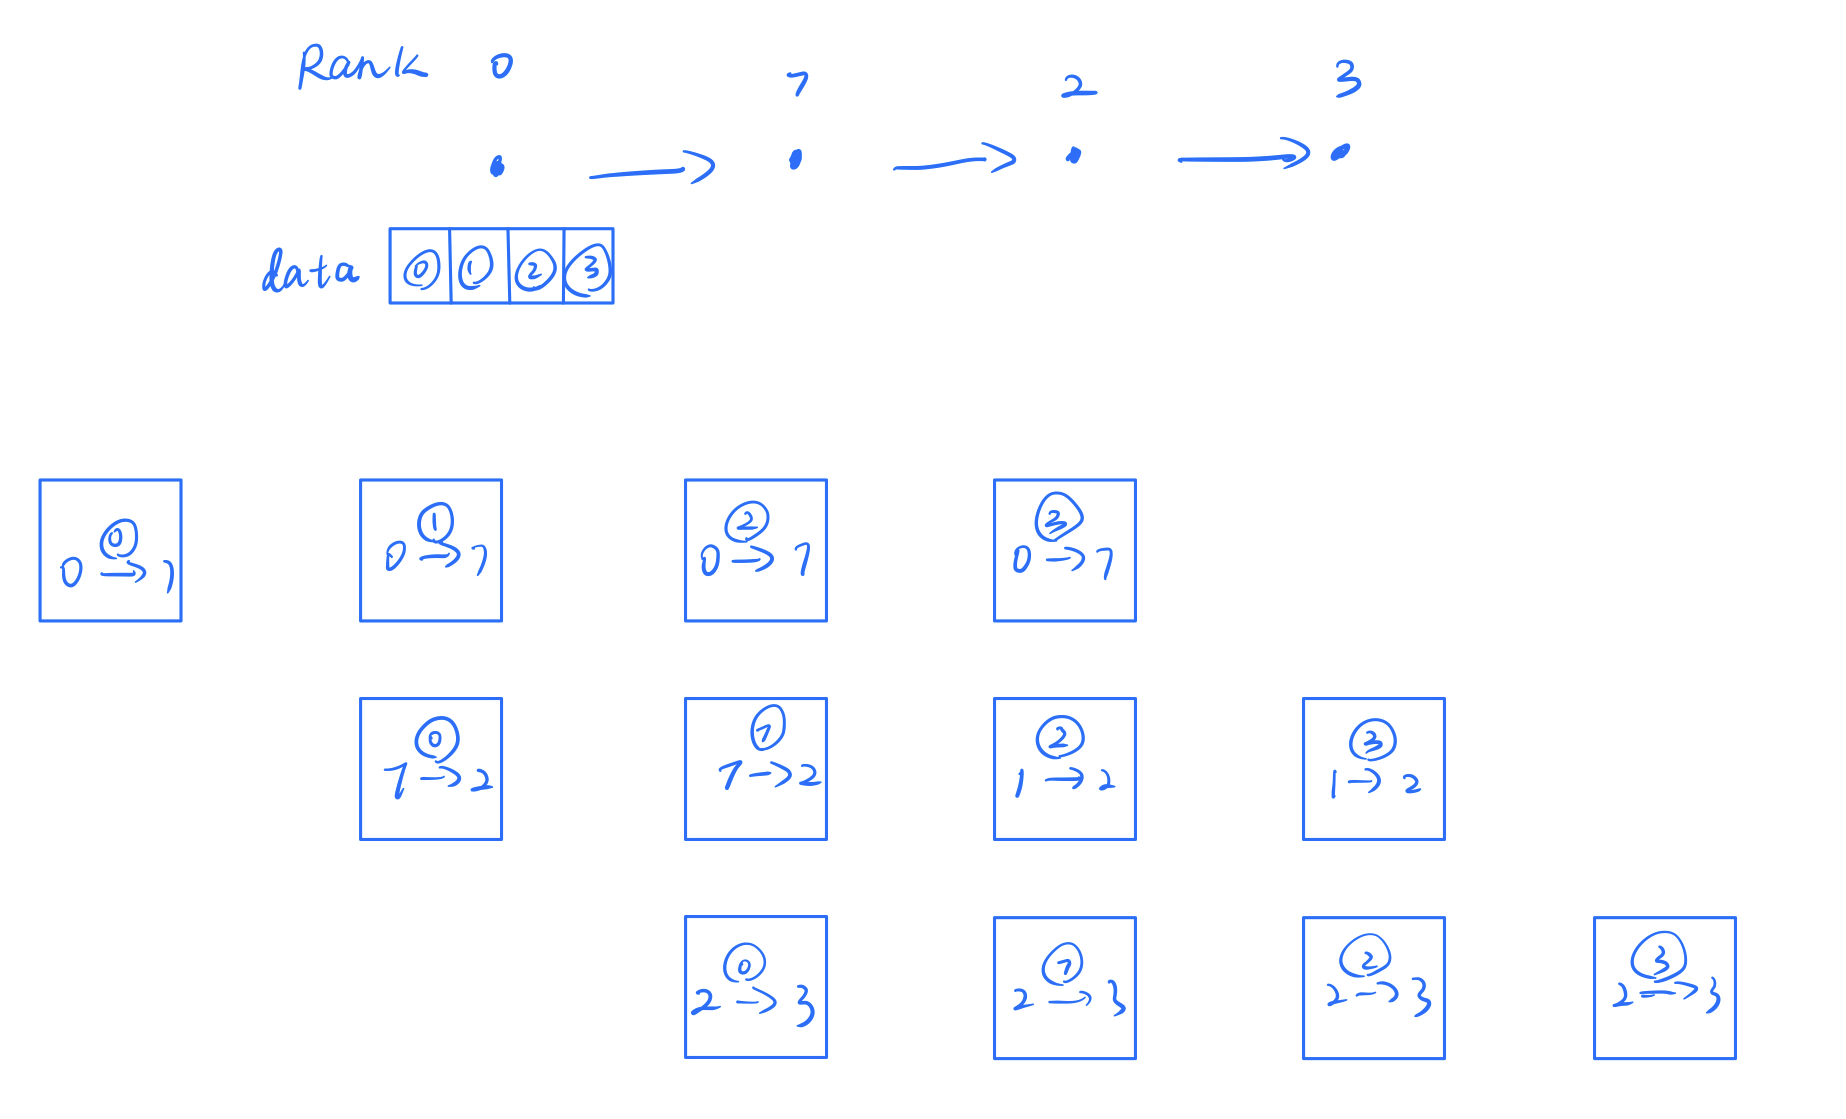
\includegraphics[width=\textwidth,height=8cm,keepaspectratio=true]{../figs/buffer_optimize.png}
  \caption{Buffer Optimization Algorithm}
  \label{fig:buffer}
\end{figure}
\\
And the result is shown in \ref{fig:buffer}.
\begin{figure}[htpb]
  \centering
  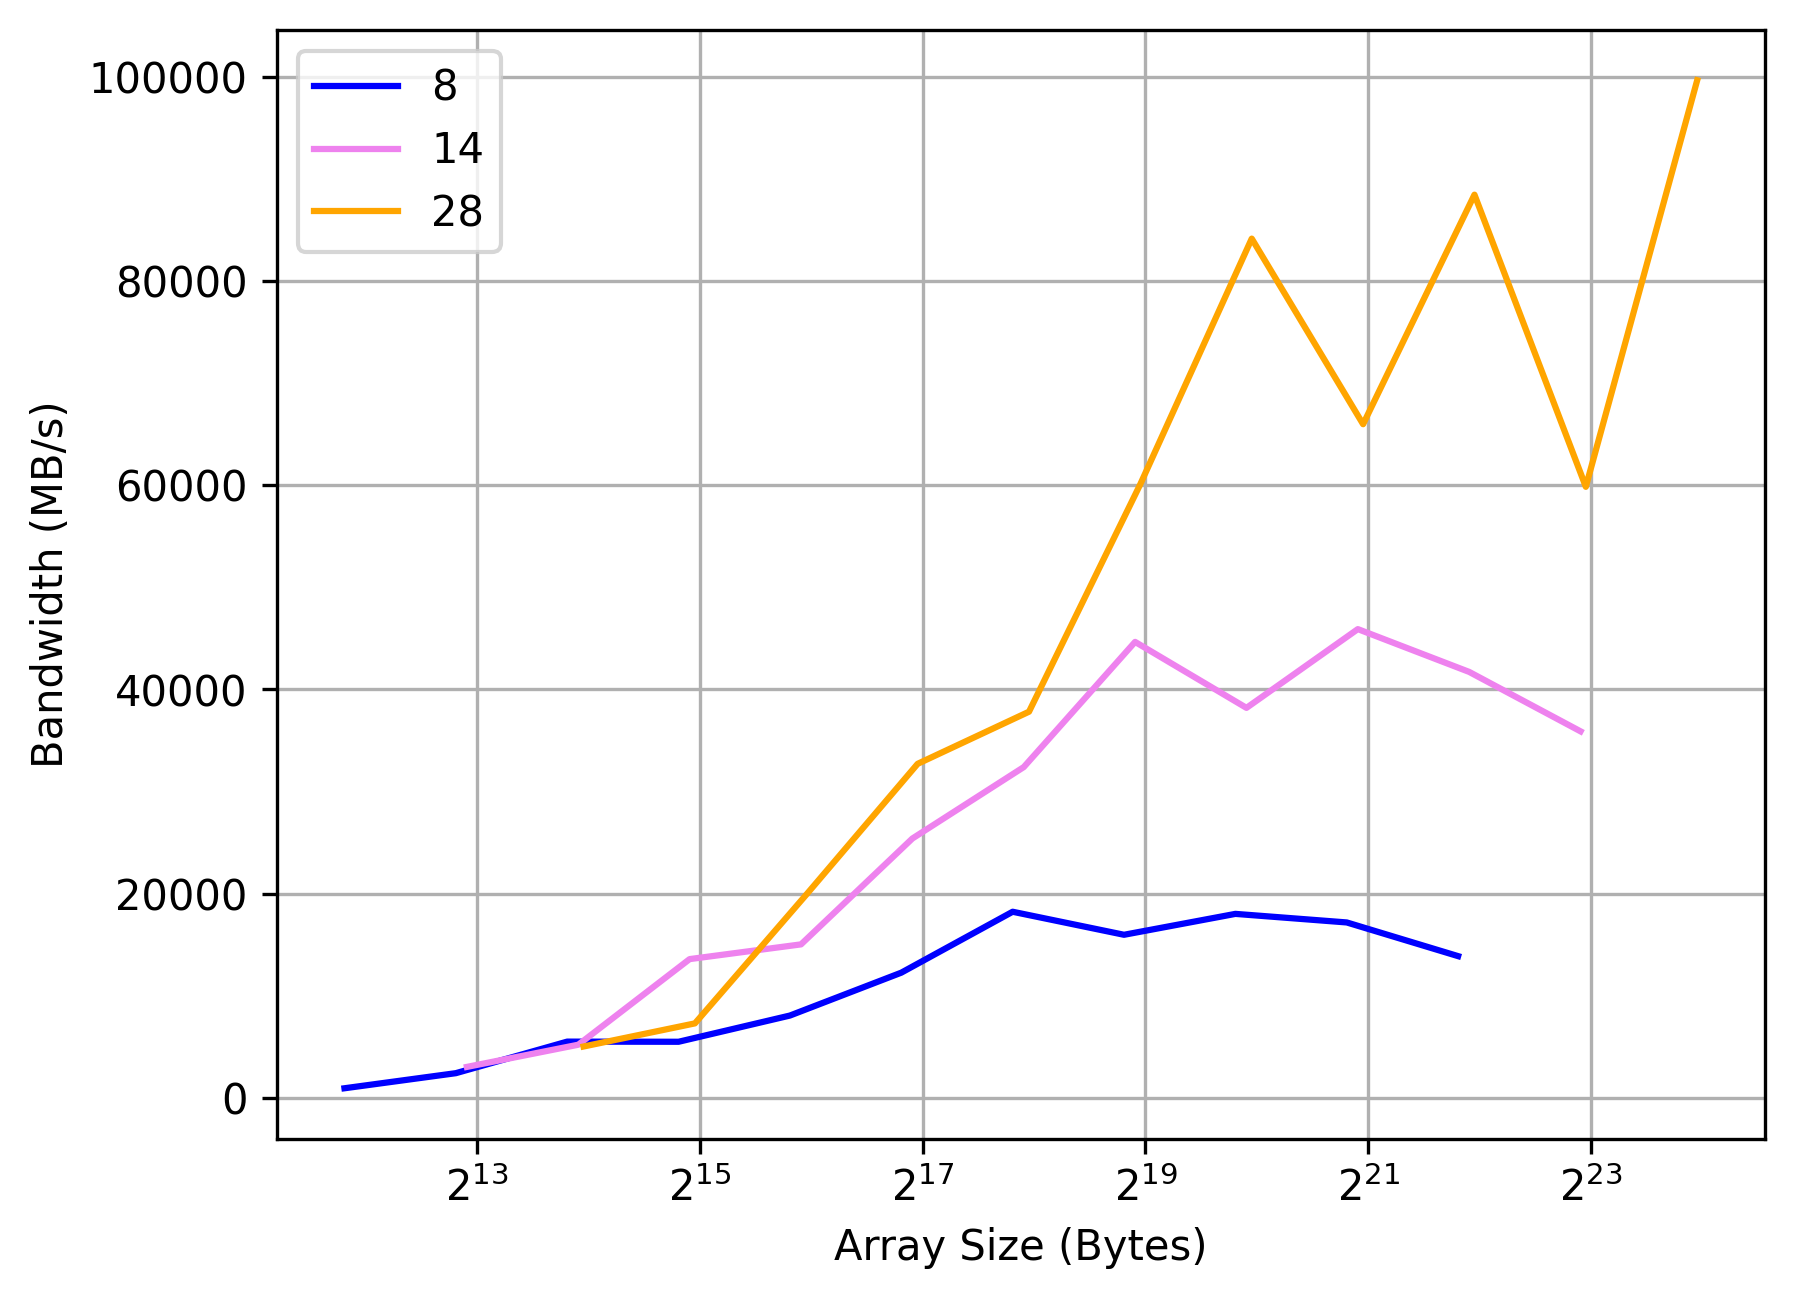
\includegraphics[width=\textwidth,height=8cm,keepaspectratio=true]{../figs/CollectiveBandwidthBuffer.png}
  \caption{Collective Network Bandwidth(buffer optimize)}
  \label{fig:buffer}
\end{figure}
Comparing the performance of these three algorithm, we saw that the tree algorithm gives us the best performance and then the buffer one, the trivial one is with no doubt the worst one.

3) Hyper mode
Since the tree algorithm optimizes the usage of bandwidth and the third algorithm optimizes the usage of buffer, combine this
two algorithm may give us a better performance. But due to the time limit we didn't implement this.\\
\begin{figure}[htpb]
  \centering
  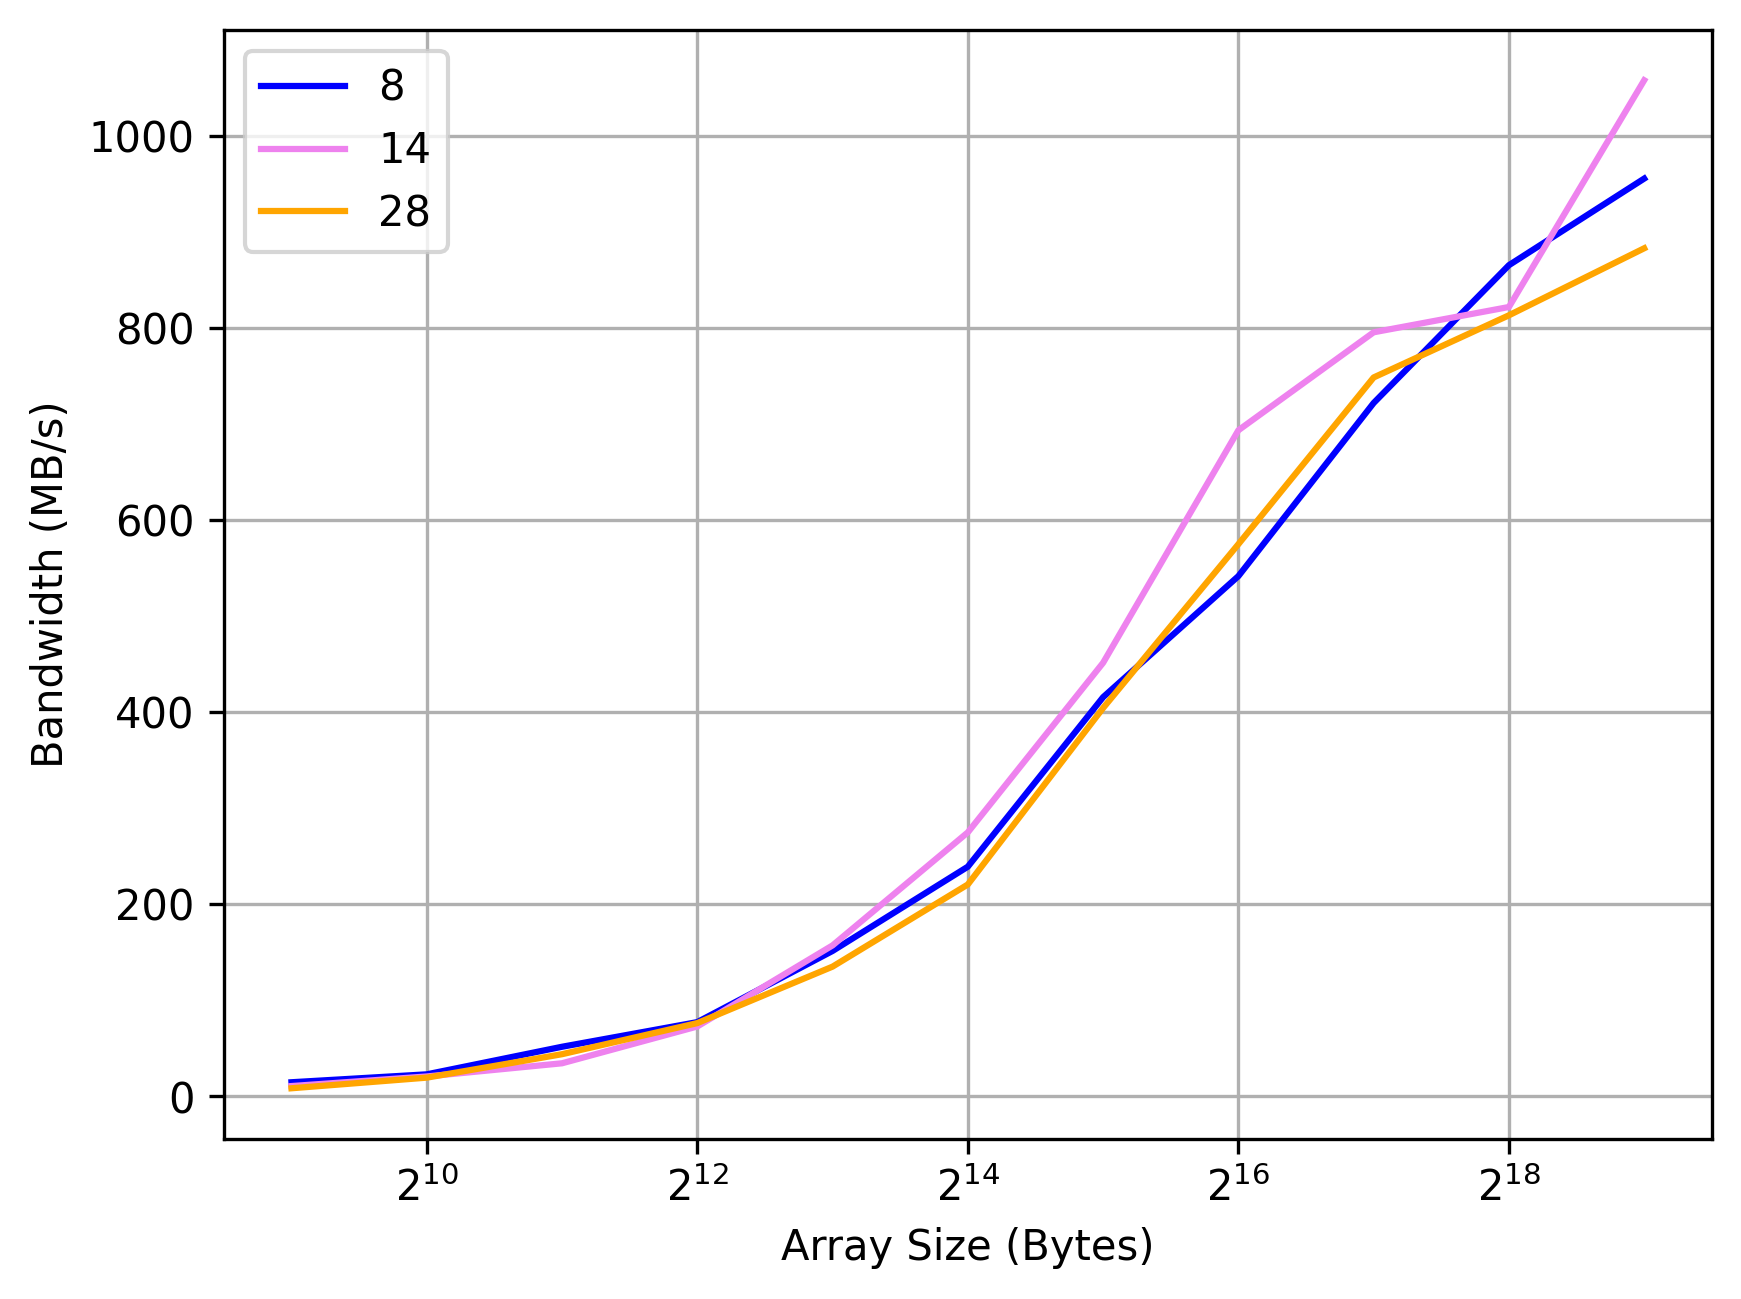
\includegraphics[width=\textwidth,height=8cm,keepaspectratio=true]{../figs/BandwidthApprox.png}
  \caption{Approximated Bandwidth(MPI\_Bcast) }
  \label{fig:MPIAppro}
\end{figure}
\\
In figure \ref{fig:MPIAppro}, we approximate the bandwidth using $B = arraySize/time$. MPI\_Bcast shows an amazing performance.
Thinking of the perfect network with M nodes, where every node has a dedicated wire to each other node.
Then when we double the process number while keeping the data size, the execution time of our application should stay the same,
and thus the bandwidth.
\section{5 Parallel CG (3P)}
\subsection{Parallelism Strategy}
\paragraph{Input and output} To avoid storing the whole data in 1 nodes, and avoid the cost of broadcas and gathering, we decided to parallelize input and output processes of the given code. For input, each process initializes each own data and stores it in a local storage. Then the program called the solver. At the end, each node write its own data into the output files. Since we don't have parallel IO yet, we write in serial, each process hold the file handler once, and write to the file. The lines in the resulted output files do not keep the same order as the output in the serial case, but it does not affect to the visuallisation, since for visuallisation we plot for each value of a point (x,y).
\paragraph{Parallel Solver}
We adjusted all helping functions so that each rank only iterates in their local domains. Besides, each the solver function, we need to have 3 communication points which call $MPI\_Allreduce$. The idea is we calculate all vector by vector locally, and broadcast and sum up the resulted double. This helps in calculating the global $delta$ and global $a$. Besides, we also need to exchange ghosh cells to update informations of the grids every time before we applies 5-points stencil to the grids. The implementation of the parallel solver is presented below.
\begin{frame}[]
%\frametitle{Inserting source code}
\lstset{language=C++,
                basicstyle=\ttfamily\footnotesize,
                keywordstyle=\color{blue}\ttfamily,
                stringstyle=\color{red}\ttfamily,
                commentstyle=\color{green}\ttfamily,
                morecomment=[l][\color{magenta}]{\#}
}
\begin{lstlisting}[frame=single]
g_product_operator(param, grid, d);
g_scale_add(param, b, d, -1.0);
memcpy(r, b, nx*ny*sizeof(double));
memcpy(d, r, nx*ny*sizeof(double));

// calculate starting norm
auto delta_local = g_dot_product(param, r, r);
double delta_global_new, delta_global_old;
MPI_Allreduce(& delta_local, &delta_global_new, 1, MPI_DOUBLE,\
			 MPI_SUM, MPI_COMM_WORLD);
delta_0 = delta_global_new*eps_squared;
residuum = (delta_0/eps_squared);

while ((needed_iters < cg_max_iterations) \
				&& (delta_global_new > delta_0))
{
    // q = A*d
    exchange_ghoshlayers(param,d);
    g_product_operator(param, d, q);
    // a = d_new / d.q
    auto a_local = g_dot_product(param, d, q);
    MPI_Allreduce(&a_local, &a, 1, MPI_DOUBLE, MPI_SUM, MPI_COMM_WORLD);
    a = delta_global_new/a;
    // x = x + a*d
    g_scale_add(param, grid, d, a);
    if ((needed_iters % 50) == 0)
    {
        memcpy(b, b_save , nx*ny*sizeof(double));
        exchange_ghoshlayers(param,grid);
        g_product_operator(param, grid, q);
        g_scale_add(param, b, q, -1.0);
        memcpy(r, b , nx*ny*sizeof(double));
    }
    else
    {
        // r = r - a*q
        g_scale_add(param, r, q, -a);
    }
    // calculate new deltas and determine beta
    delta_global_old = delta_global_new;
    delta_local = g_dot_product(param, r, r);
    MPI_Allreduce(&delta_local, &delta_global_new, 1, MPI_DOUBLE,\
    				MPI_SUM, param->comm_2d);
    beta = delta_global_new/delta_global_old;
    // adjust d
    g_scale(param, d, beta);
    g_scale_add(param, d, r, 1.0);
    residuum = delta_global_new;
    needed_iters++;
}
\end{lstlisting}
\end{frame}
\paragraph{Ghosh cell exchange}
Each rank has 4 neighbors, when we want to exchange ghoshcells, the rank needs to communicate with these fours. Communications with top and bottom neighbors are pretty simple since the data is contiguous in memory. But, for the case with left and rights, since we need to to send columns data but data was stored in row-major, we need to define an additional data type with $MPI\_Type\_vector$. The ghosh cell exchanges is presented in the code below.
\begin{frame}[]
%\frametitle{Inserting source code}
\lstset{language=C++,
                basicstyle=\ttfamily\footnotesize,
                keywordstyle=\color{blue}\ttfamily,
                stringstyle=\color{red}\ttfamily,
                commentstyle=\color{green}\ttfamily,
                morecomment=[l][\color{magenta}]{\#}
}
\begin{lstlisting}[frame=single]
// Exchange top most row to the top neighbors:
MPI_Sendrecv(grid + (ny-2)*nx, nx, MPI_DOUBLE, param->topo_top, toptag,
        grid, nx, MPI_DOUBLE, param->topo_bottom, toptag,
        MPI_COMM_WORLD, MPI_STATUS_IGNORE);

// Exchange row most row to the bottom neighbors:
MPI_Sendrecv(grid + nx, nx, MPI_DOUBLE, param->topo_bottom, downtag,
        grid + (ny-1)*nx, nx, MPI_DOUBLE, param->topo_top, downtag,
        MPI_COMM_WORLD, MPI_STATUS_IGNORE);

// Data type for sending columns
MPI_Datatype column_type;
MPI_Type_vector(ny, 1, nx, MPI_DOUBLE, &column_type);
MPI_Type_commit(&column_type);
For that
// Exchange left most column to the left neighbors:
MPI_Sendrecv(grid + 1, 1, column_type, param->topo_left, lefttag, 
        grid + nx - 1, 1, column_type, param->topo_right, lefttag, 
        MPI_COMM_WORLD, MPI_STATUS_IGNORE);
// Exchange right most column to the right neighbors:
MPI_Sendrecv(grid + nx - 2, 1, column_type, param->topo_right, righttag,
        grid , 1, column_type, param->topo_left, righttag, 
        MPI_COMM_WORLD, MPI_STATUS_IGNORE);
\end{lstlisting}
\end{frame}
\subsection{Results and Discussions}
\paragraph{Validation}
The program was ran with gridsize = 0.001 and eps = 0.0000001 on the local computer. The output then visualized with gnuplot. Resulted picture is as blow:

\begin{figure}[htpb]
  \centering
  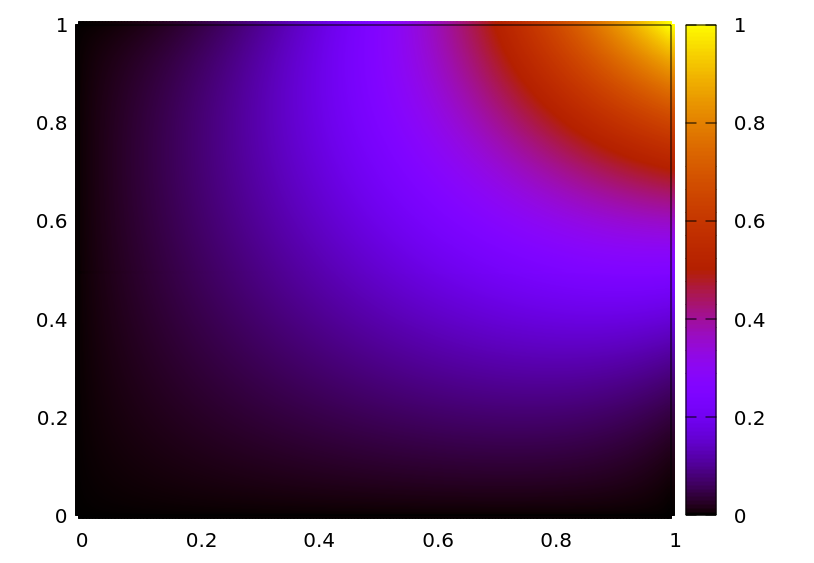
\includegraphics[width=\textwidth,height=8cm,keepaspectratio=true]{../figs/solution_mpi.png}
  \caption{Visualization of solution with parallel solver}
  \label{fig:sol1}
\end{figure}

The number of required iterations and final residum remained unchanges when we ran the program with different number of cores and different MPI topology (Table \ref{table:topo1}). The Figure \ref{fig:sol1} showed the expected solution. Thus this parallel solver is reliable.

\paragraph{Performance of different process-grids}
We tested the program on 1 node of CM2 with 28 MPI processes, 1 process/core. The gridsize is 0.0005 and eps is 0.0005. The table below presented the performance in respect to different MPI topology.
\begin{center}
\begin{tabular}{ |c|c|c|c|c|c| } 
 \hline
nMPI&TopoX&   TopoY& nIterations&     Residum &    Time \\
 \hline
 28 &  1  &		28 &     1717   & 1.24881e-17 &    5.41372\\
28  & 2   &		14 &     1717   & 1.24881e-17 &    5.30194\\
28  & 4   &		7  & 1717    	&1.24881e-17  &   5.30789\\
28  & 7   &		4  & 1717    	&1.24881e-17  &   5.36031\\
28  & 14  &    2   &1717    	&1.24881e-17  &   5.43706\\
28  & 28  &    1   &1717    	&1.24881e-17  &   5.72815\\
 \hline

\end{tabular}
\label(table:topo1)
\end{center}
Regarding the runtime, there is no significant differences between different topology choices. The (2x14) and (4x7) seems to have the best performance. Normally, we would expected the topology which comes near to the shape of a square will performance the best, since it's optimal for the amount we need to exchange in each boundary, at the same time optimal for collective operations. In our case, since we have 28 cores, (4x7) is the most close to "a square" that we could get.

\paragraph{Performance of different grid-sizes}
We performed the test with different grid sizes. For this we used 1 nodes which has 28 tasks, 1 task/core. The results are presented in Figure \ref{fig:grid1} and \ref{fig:grid2}. 

\begin{figure}[htpb]
  \centering
  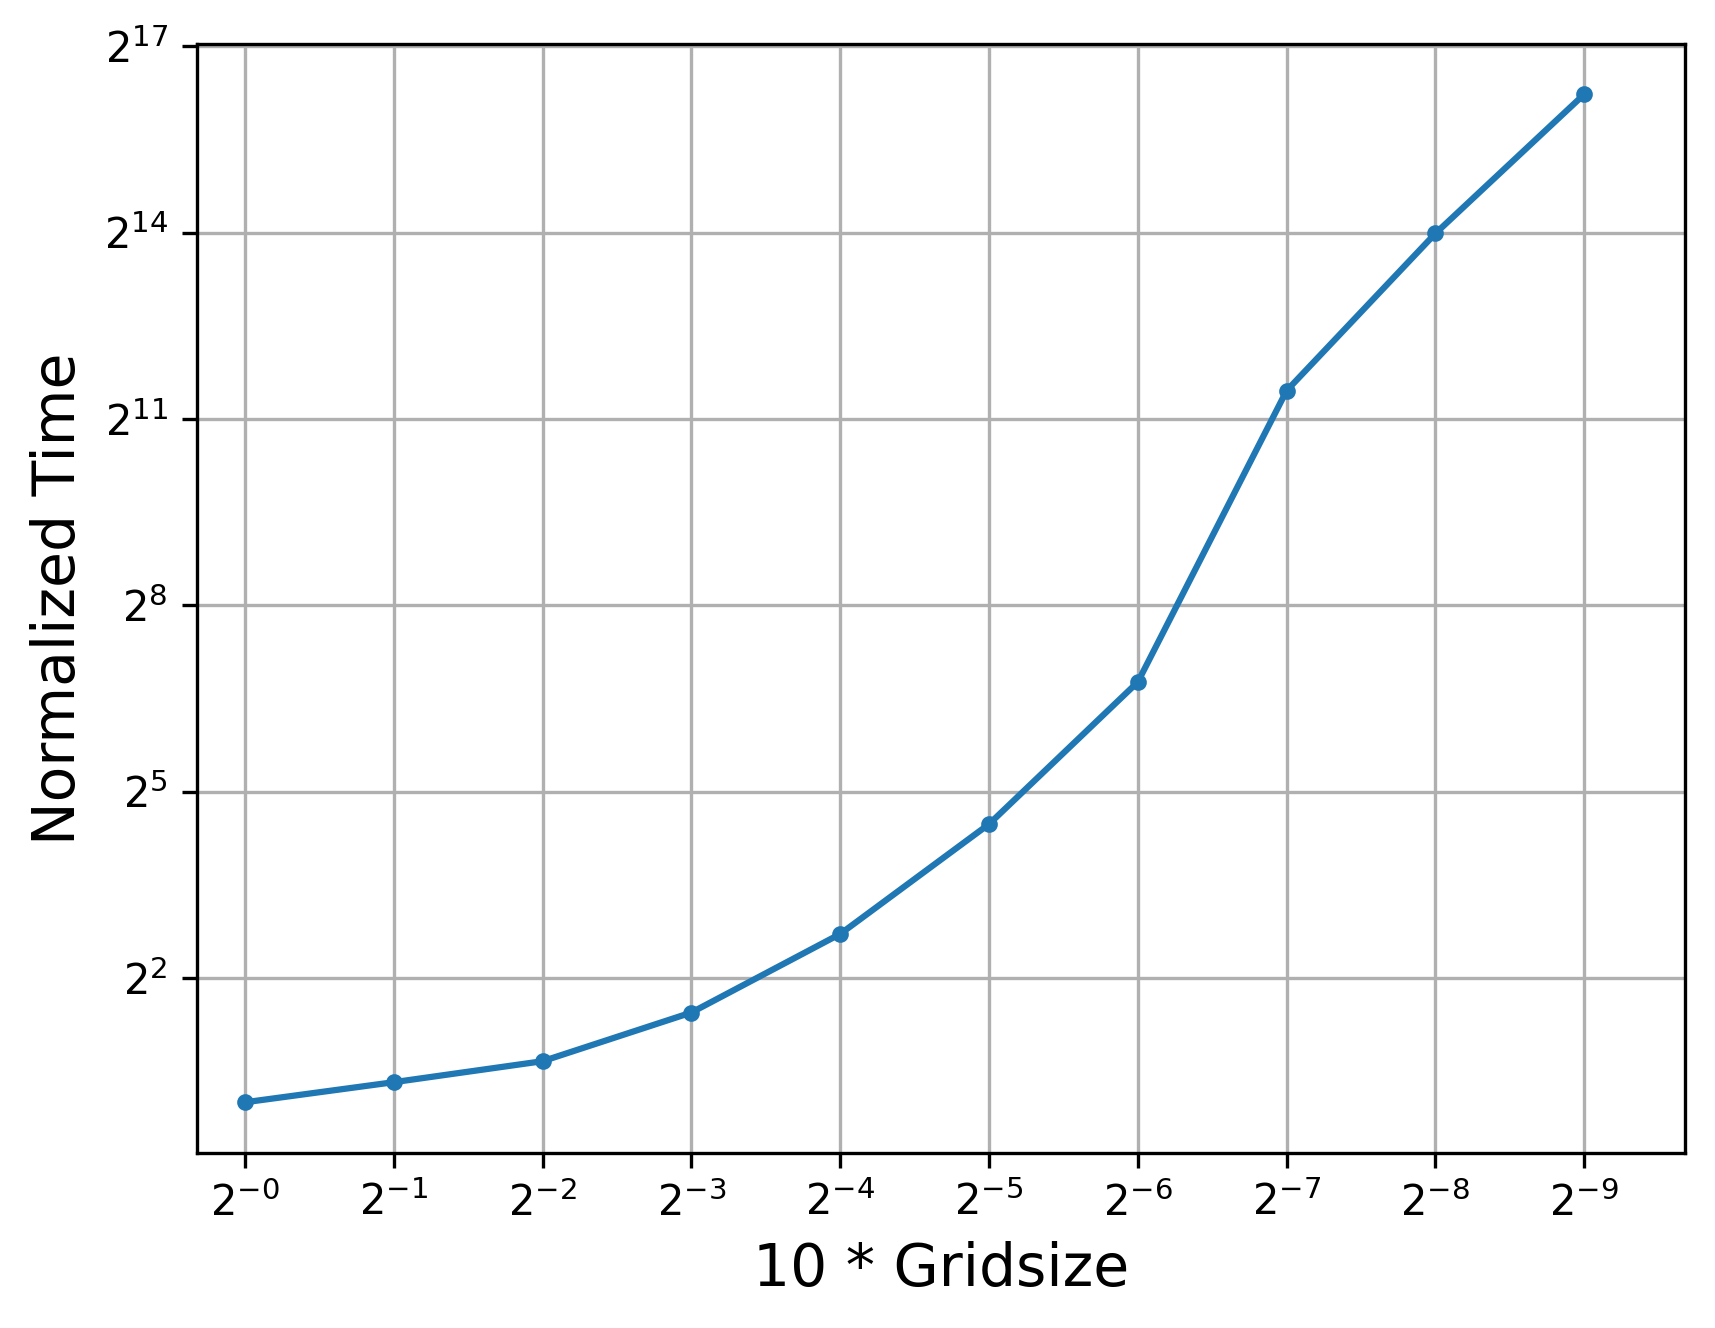
\includegraphics[width=\textwidth,height=8cm,keepaspectratio=true]{../figs/5_gridsizes_1.png}
  \caption{Normalized runtime of different grid sizes}
  \label{fig:grid1}
\end{figure}
\begin{figure}[htpb]
  \centering
  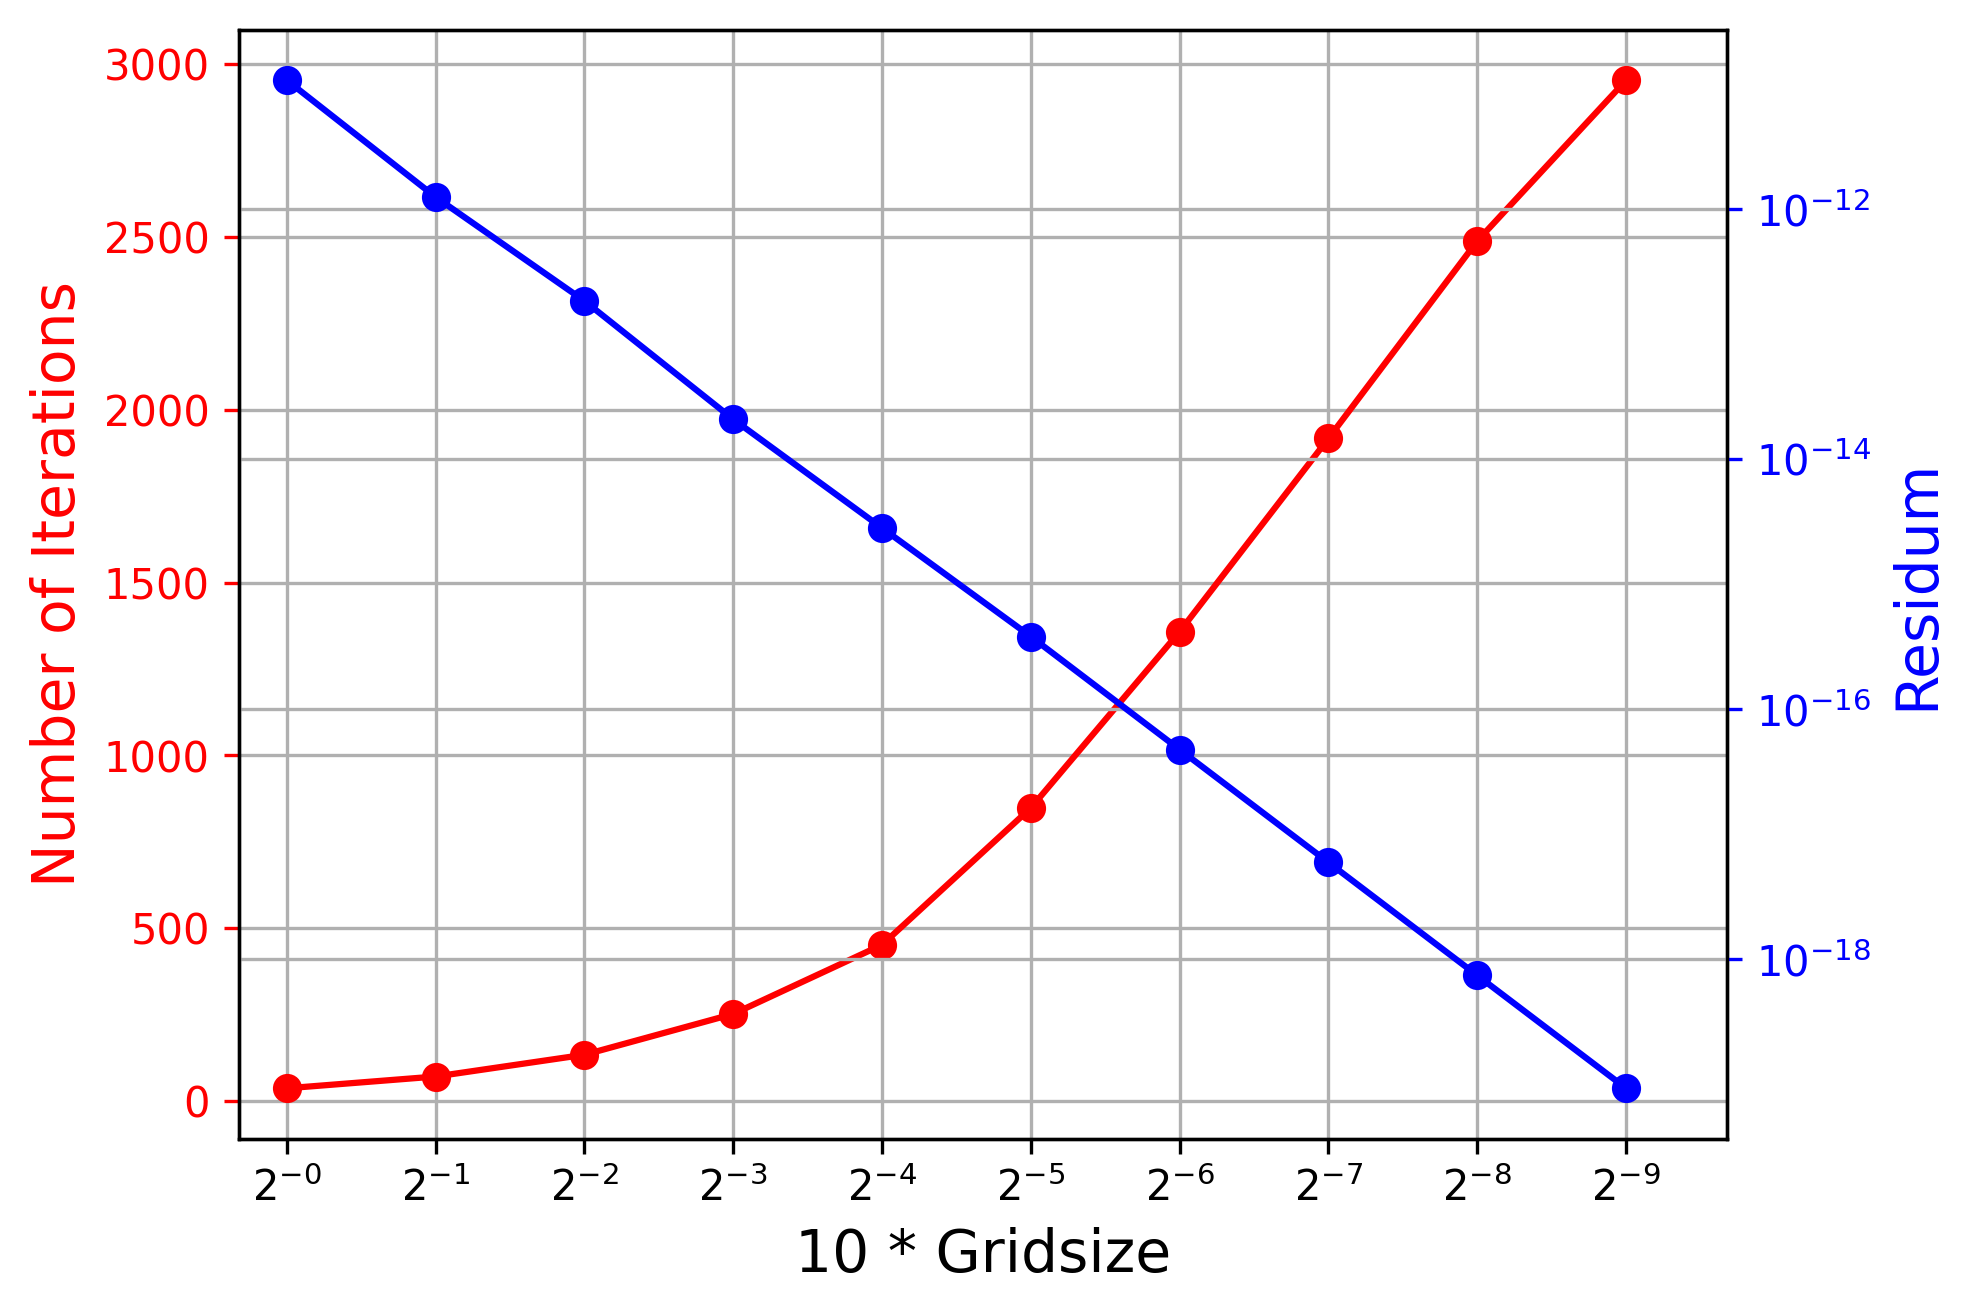
\includegraphics[width=\textwidth,height=8cm,keepaspectratio=true]{../figs/5_gridsizes_2.png}
  \caption{Number of iterations and final residual vs. different grid sizes}
  \label{fig:grid2}
\end{figure}

From these two figures, we can see that the run time is increased proportionally to the number of required iterations so that the simulation converged. Besides, both runtime and number of required iterations seems to increase exponentially when we decrease grid sizes. When we decreased the grid size by 2, the runtime increased about 4-8 times depends on the problem sizes. 4 times would be a reasonable number since when we decrease the grid size by 2, the number of grid points in each dimension increases by 2, thus the number of total grid points increase by 4. However, this performance is also affected by cache-effects. When we have big grid sizes, we have small number of total grid points, this the data still can fit into caches. It's not the case when we have smaller grid sizes. Thus the time can increase more than 4 times.

For the final residuals, it decrease proportionally in respect to the grid sizes. This is due to the criteria we set as a stopping condition. 

\paragraph{Strong-scale test in 1 node}
We use number of tasks ranging from 1 to 28, each task binds to 1 core. The result is in Figure \ref{fig:strong1}

\begin{figure}[htpb]
  \centering
  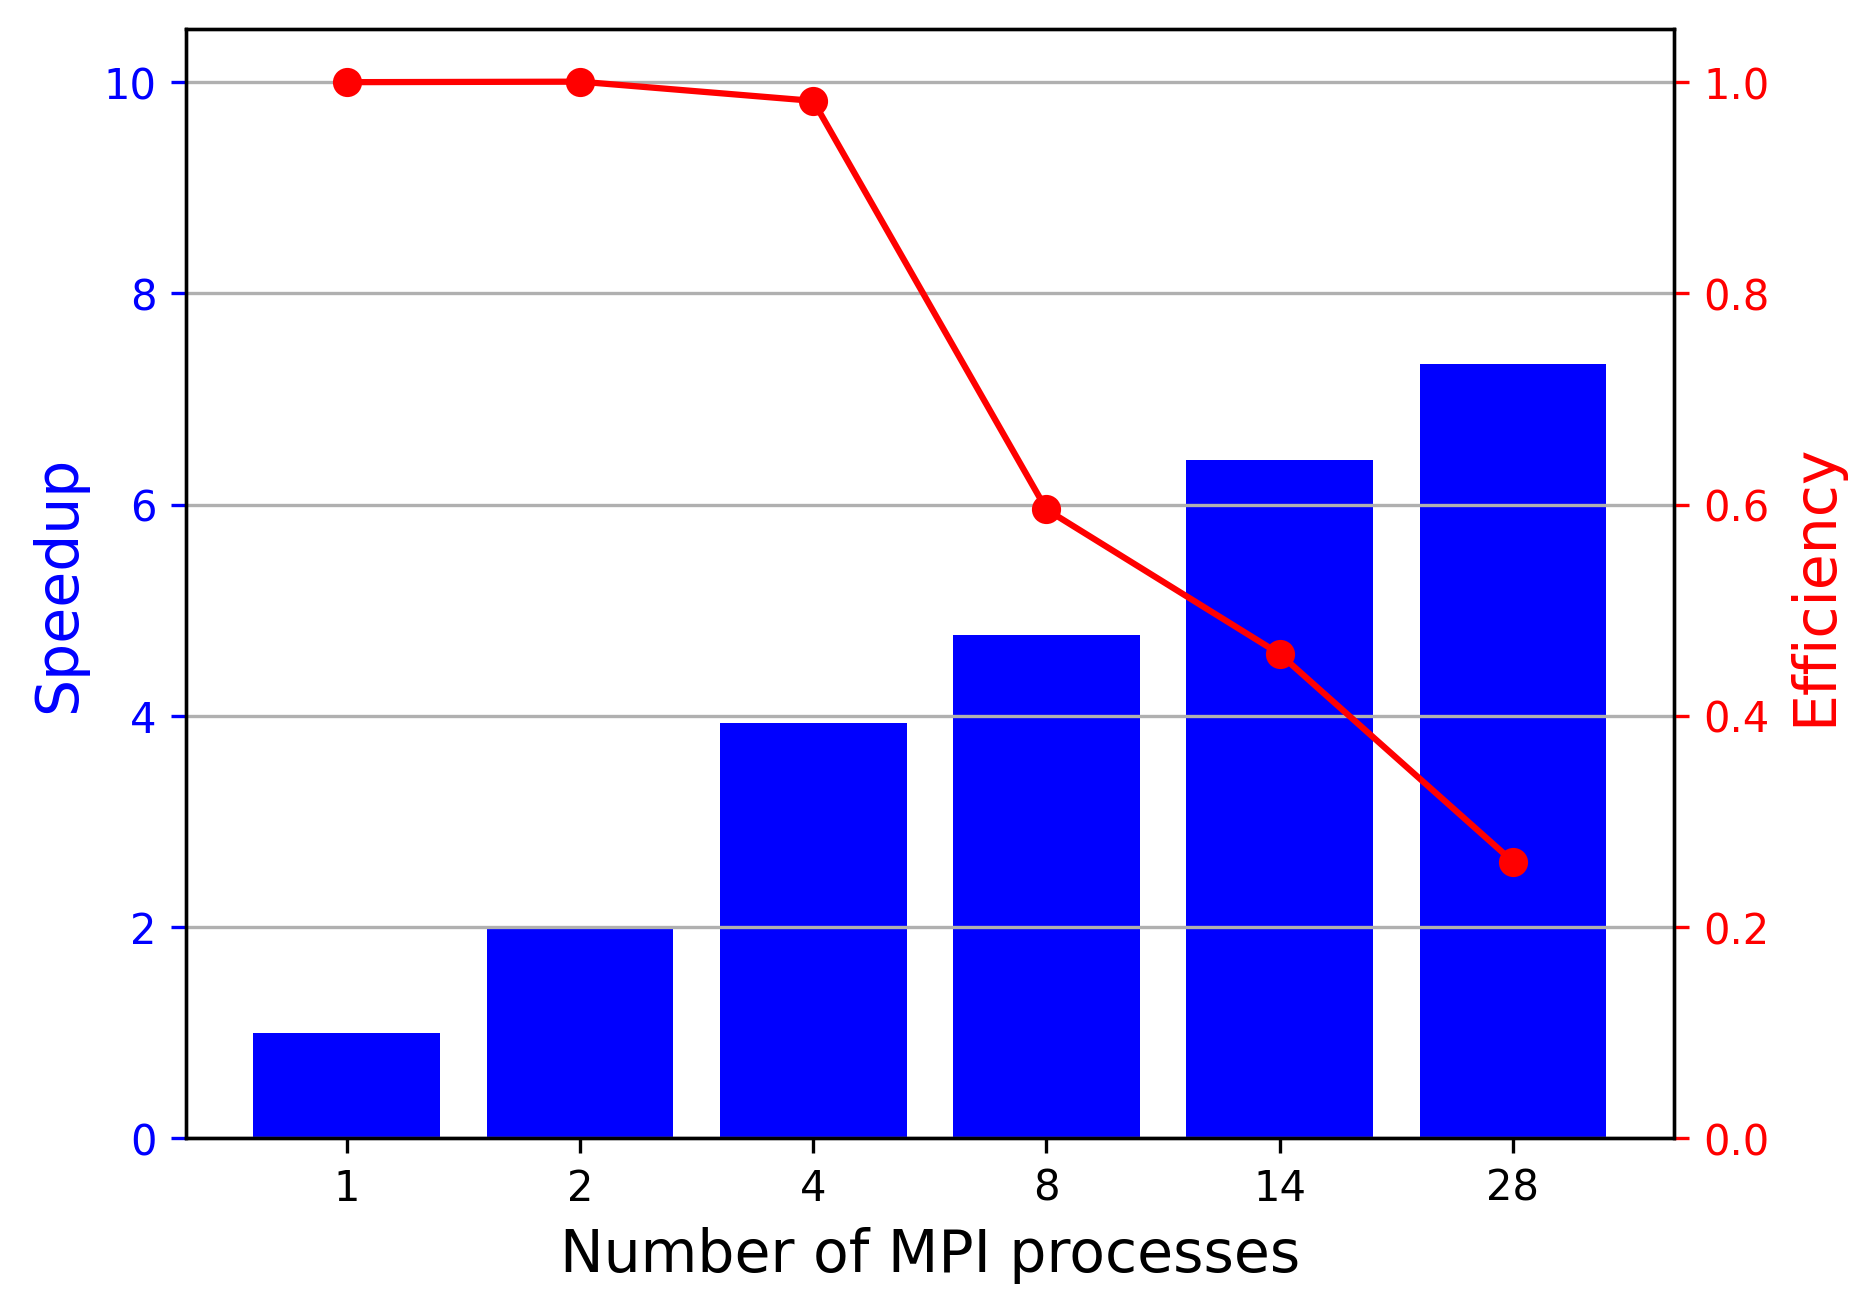
\includegraphics[width=\textwidth,height=8cm,keepaspectratio=true]{../figs/5_strong_1.png}
  \caption{Strong-scale performance in 1 node, grid size = 0.00025}
  \label{fig:strong1}
\end{figure}
With a fix problem size (grid size = 0.00025), from 1 MPI task to 4 MPI tasks, we observed a linear-scaling which is good. However, when the number of MPI processes goes over 8, the speed up is not that good anymore. This trend is also revealed by the Efficiency line, while it kept steady at 1 from 1-4 processes, and dropped down when having more processes. 

This trend is reasonable, since when we use 28 MPI processes in 1 node, the cost of communications overshadows the computation that can be done in parallel. Besides, such communications can be limited by the bandwidth and latency of the communication networks (even in side of 1 node).
   
\paragraph{Strong-scale test in 4 nodes}
We kept the same problem size as the above test (grid size = 0.00025) and increases number of using cores beyond a node. The results are shown in the Figure \ref{fig:strong2}

\begin{figure}[htpb]
  \centering
  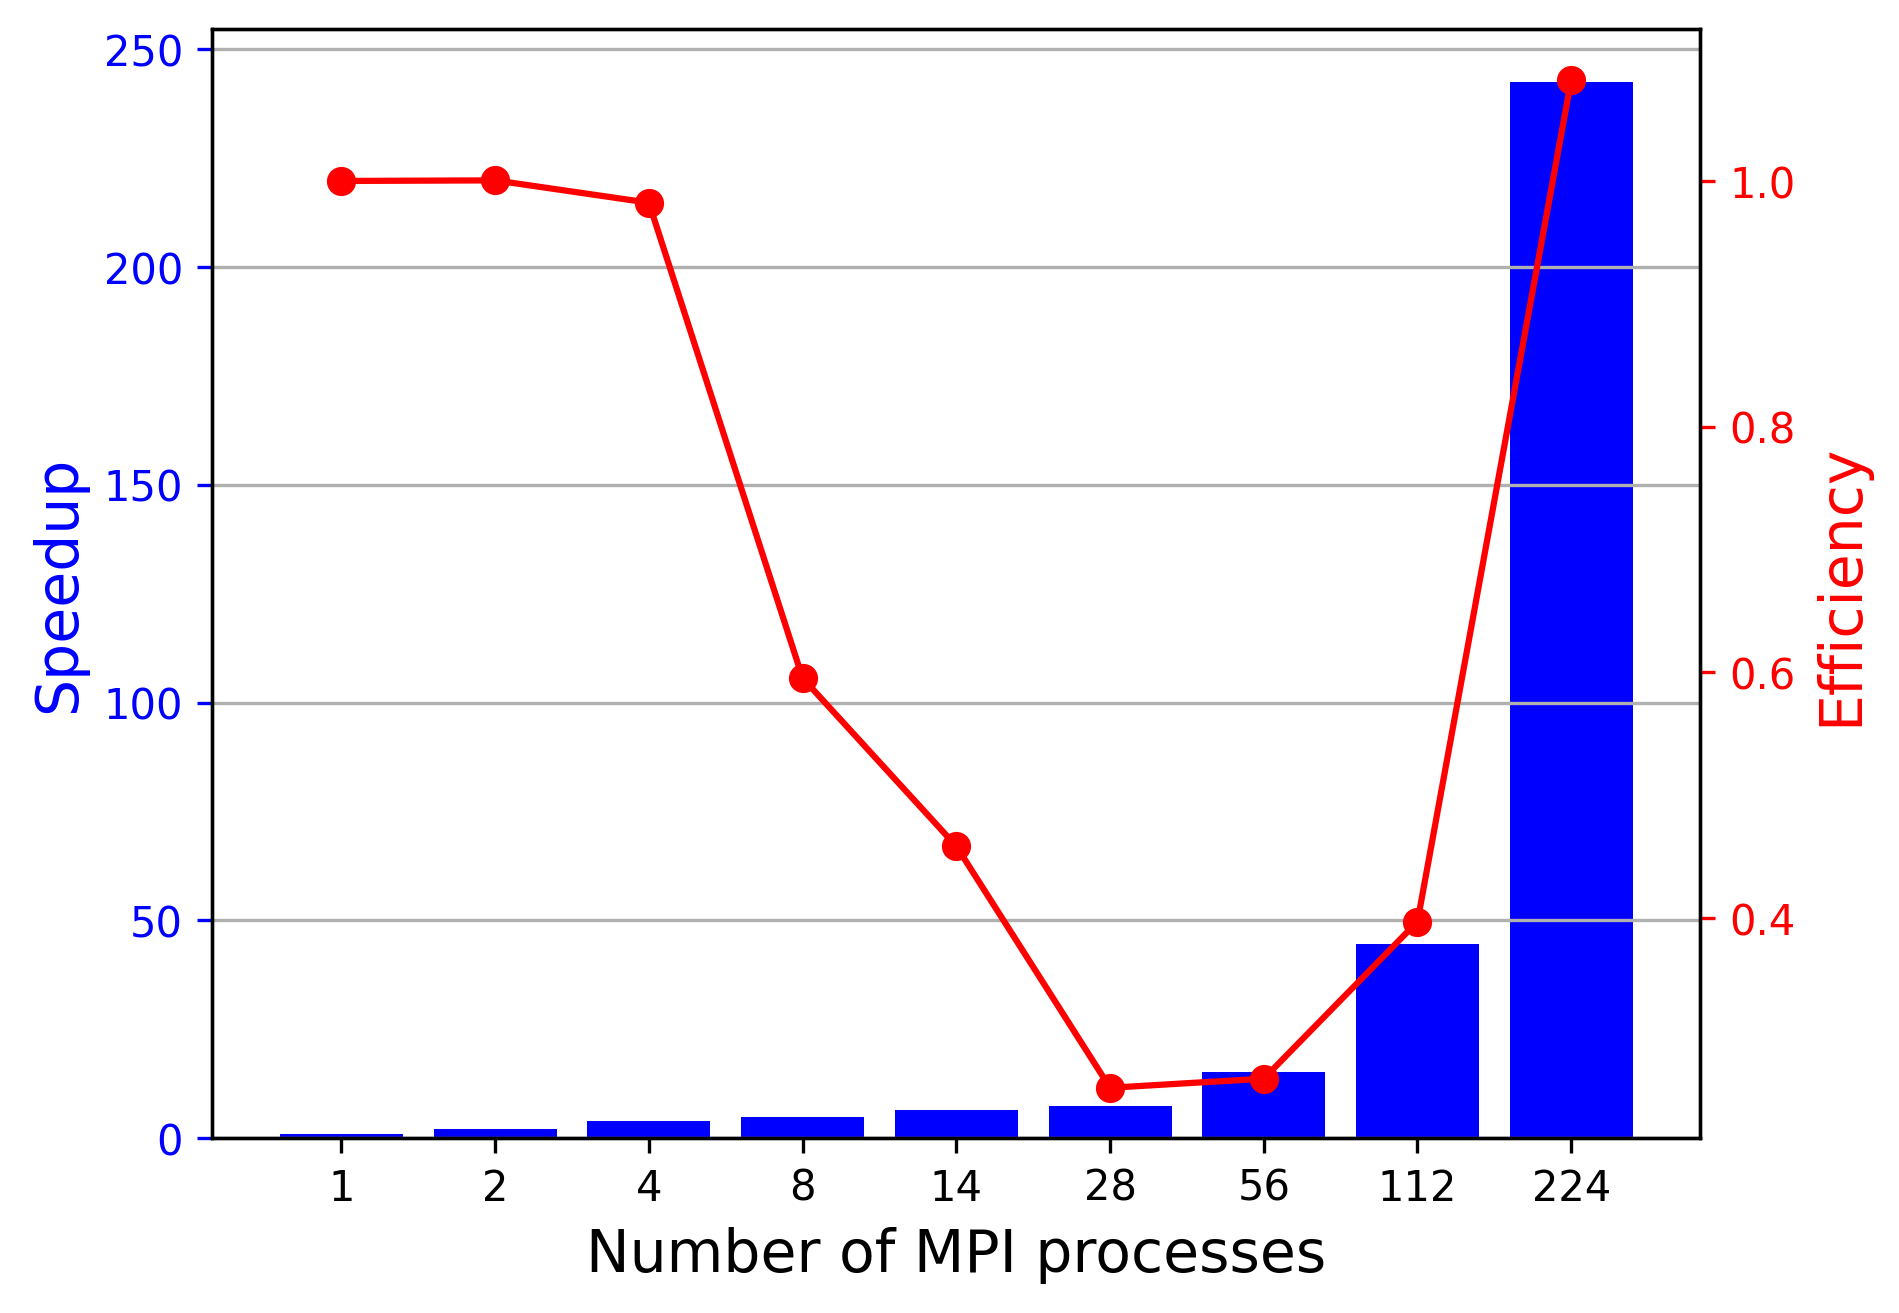
\includegraphics[width=\textwidth,height=8cm,keepaspectratio=true]{../figs/5_strong_4.png}
  \caption{Strong-scale performance in 4 node, grid size = 0.00025}
  \label{fig:strong2}
\end{figure}

Interestingly, when going beyond 1 node, we observed a super-linear scaling, especially in the test with 224 MPI processes on 4 nodes, the speedup is 242 times, and the efficiency is 1.08. This might be due to the reason that we a fixed problem size, when we have more cores, then the sub-problem can be fit into the processes caches, thus the efficiency is even better then the single core test. 

To verify this, we increased the problem size further by decreasing the grid size to 0.0001. We tested with 4 nodes and the normalized speedup is presented below in Figure \ref{fig:strong3}.   

\begin{figure}[htpb]
  \centering
  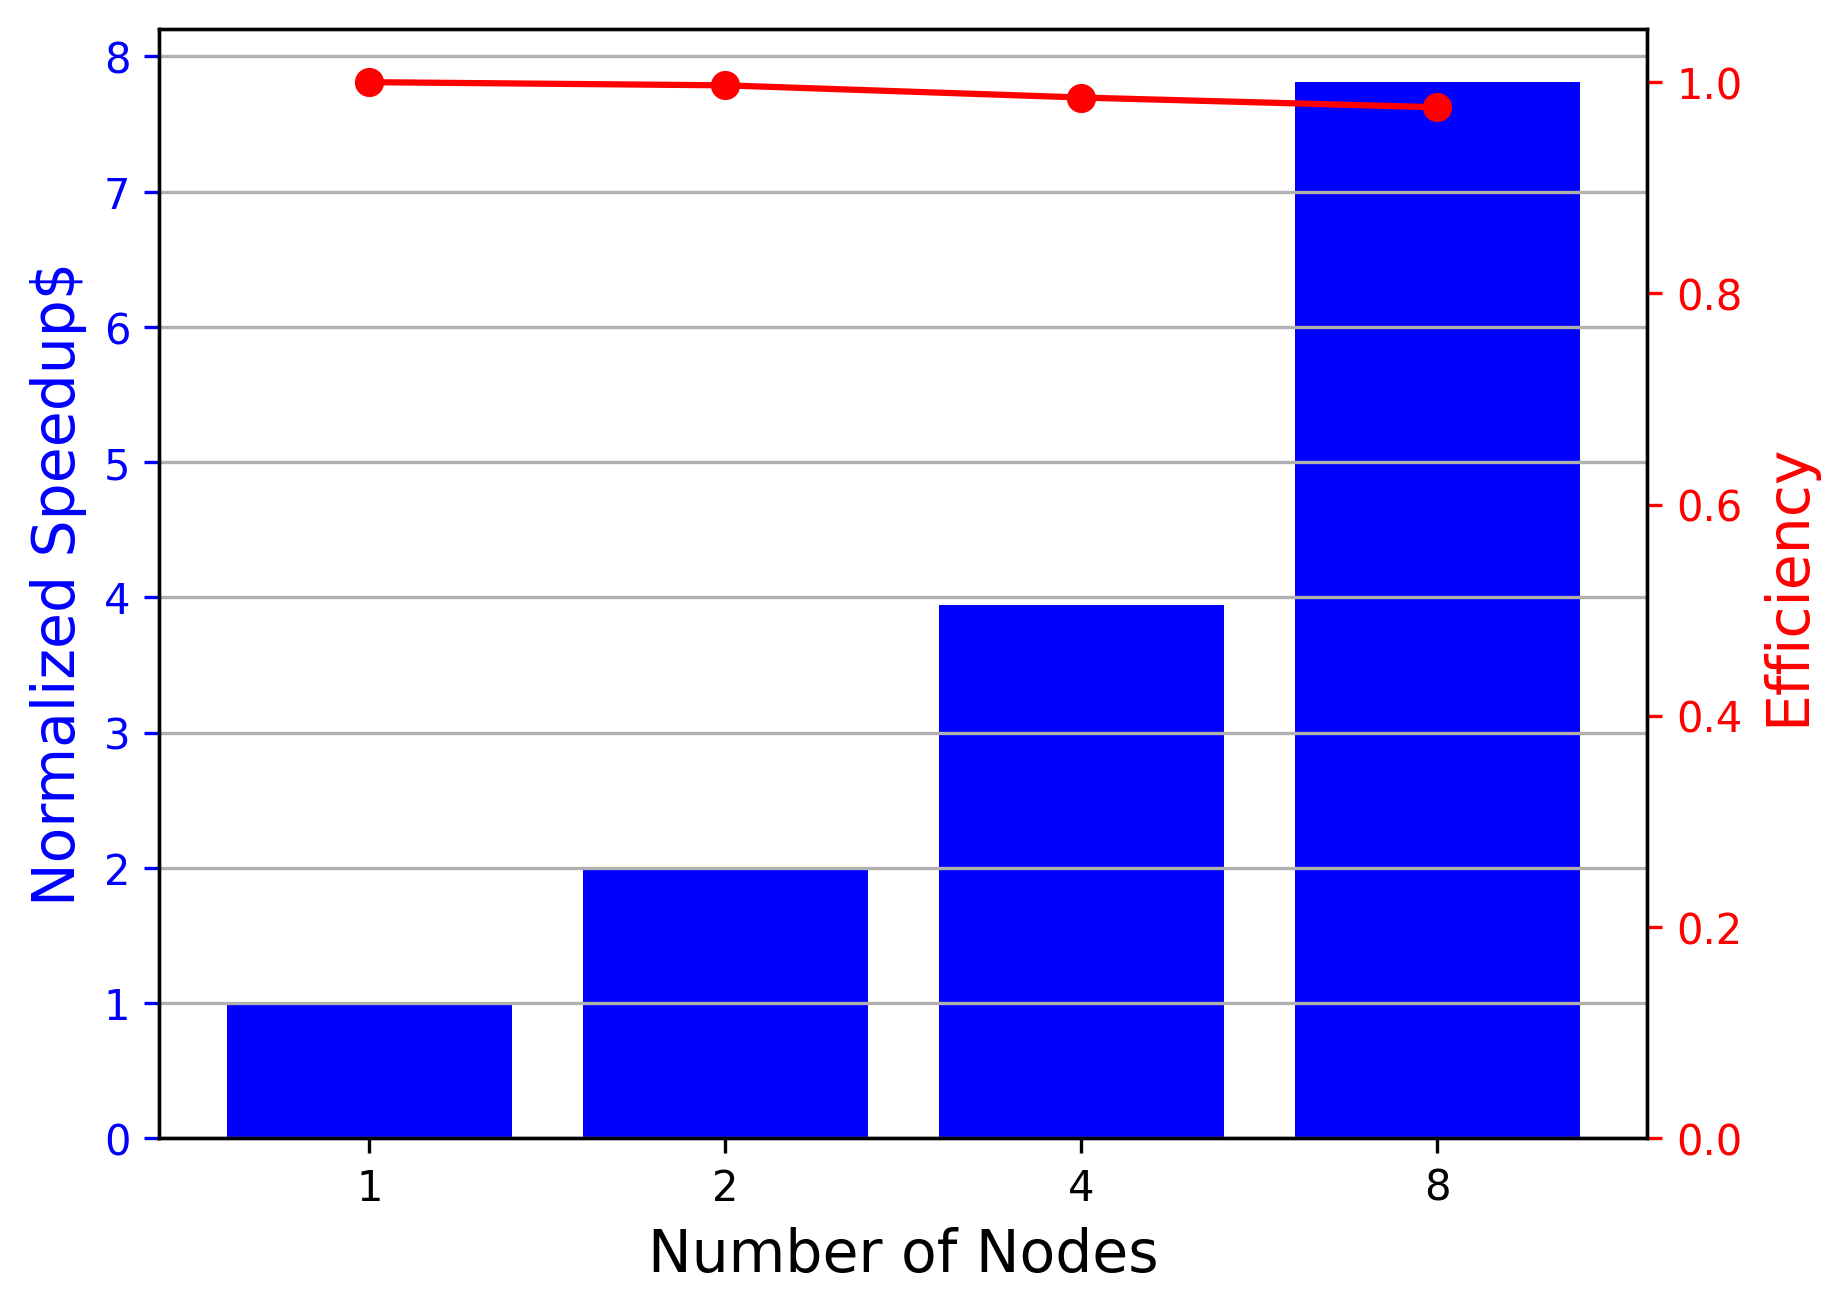
\includegraphics[width=\textwidth,height=8cm,keepaspectratio=true]{../figs/5_strong_5.png}
  \caption{Strong-scale performance in 4 node, grid size = 0.0001}
  \label{fig:strong3}
\end{figure}
Here the super-linear scaling effect is disappear. The program scales nicely in respect to number of nodes and the efficiency remains almost constant around 1. This means our prediction for super-linear scale for the previous test is correct. 

\subsection{Future Optimisation}
Due to limitation in time, we could not manage to optimize the code further. Possible optimizations are listed below:  
\begin{itemize}
	\item Parallelizing output with MPI-IO ($MPI\_File$)
	\item Overlapping communication and computation.
\end{itemize}
\medskip
%\printbibliography
\bibliography{myref}{}
\bibliographystyle{plain}

\end{document}
